\documentclass[a4paper,11pt]{article}

\usepackage{iftex}
\ifPDFTeX
  \usepackage{vntex}
  \usepackage[utf8]{inputenc}
\else
  \usepackage{fontspec}
  \setmainfont{DejaVu Serif}
  \usepackage{polyglossia}
  \setdefaultlanguage{vietnamese}
\fi

\usepackage{a4wide,amssymb,latexsym,multicol,array,hhline,fancyhdr}
\usepackage{booktabs}
\usepackage{amsmath}
\usepackage{lastpage}
\usepackage{enumerate}
\usepackage{color}
\usepackage{graphicx}
\usepackage{tabularx, caption}
\usepackage{multirow}
\usepackage{rotating}
\usepackage{geometry}
\geometry{a4paper, total={170mm,245mm}, left=20mm, right=20mm, top=25mm, bottom=25mm}
\usepackage{setspace}
\usepackage{float}
\usepackage{tikz}
\usepackage{listings}
\usepackage{longtable}
\usepackage{subcaption}
\usepackage{url}
\usepackage{hyperref}
\hypersetup{
  urlcolor=blue,
  linkcolor=black,
  citecolor=black,
  colorlinks=true
}

\newtheorem{theorem}{{\bf Định lý}}
\newtheorem{property}{{\bf Tính chất}}
\newtheorem{proposition}{{\bf Mệnh đề}}
\newtheorem{corollary}[proposition]{{\bf Hệ quả}}
\newtheorem{lemma}[proposition]{{\bf Bổ đề}}

\setlength{\headheight}{40pt}
\pagestyle{fancy}
\fancyhead{}
\fancyhead[L]{
 \begin{tabular}{rl}
    \begin{picture}(25,15)(0,0)
    \put(0,-8){
\includegraphics[width=8mm, height=8mm]{hcmut.png}}
   \end{picture}&
	\begin{tabular}{l}
		\textbf{\ttfamily Trường Đại Học Bách Khoa Tp.Hồ Chí Minh}\\
		\textbf{\ttfamily Khoa Khoa Học và Kỹ Thuật Máy Tính}
	\end{tabular} 	
 \end{tabular}
}
\fancyhead[R]{
	\begin{tabular}{l}
		\tiny \bf \\
		\tiny \bf 
	\end{tabular}  }
\fancyfoot{}
\fancyfoot[L]{\scriptsize \ttfamily Báo cáo môn CO5177 — Niên khoá 2026-2027}
\fancyfoot[R]{\scriptsize \ttfamily Trang {\thepage}/\pageref{LastPage}}
\renewcommand{\headrulewidth}{0.3pt}
\renewcommand{\footrulewidth}{0.3pt}

\setcounter{secnumdepth}{4}
\setcounter{tocdepth}{3}

\begin{document}

\begin{titlepage}
\begin{center}
ĐẠI HỌC QUỐC GIA THÀNH PHỐ HỒ CHÍ MINH \\
TRƯỜNG ĐẠI HỌC BÁCH KHOA \\
KHOA KHOA HỌC - KỸ THUẬT MÁY TÍNH 
\end{center}

\vspace{1cm}

\begin{figure}[H]
\begin{center}

\includegraphics[width=3cm]{hcmut.png}
\end{center}
\end{figure}

\vspace{0.8cm}

\begin{center}
\begin{tabular}{c}
	\multicolumn{1}{l}{\textbf{{\Large CO5177 — Nền tảng lập trình cho PTDL}}}\\
	~~\\
	\hline
	\\
	\multicolumn{1}{l}{\textbf{{\Large BÁO CÁO BÀI TẬP LỚN}}}\\
	\\
	\textbf{{\Huge Nhóm SlightSeek}}\\
	\\
	\textbf{{\Large Nghiên cứu và Thực nghiệm trên Ba Loại Dữ liệu:}}\\
	\textbf{{\Large Dữ liệu Bảng (Tabular), Ảnh (Image) và Văn bản (Text)}}\\
	\\
	\hline
\end{tabular}
\end{center}

\vspace{2cm}

\begin{table}[H]
\centering
\begin{tabular}{rrl}
\hspace{2cm} & \textbf{Giảng viên hướng dẫn:} & TS. Lê Thành Sách \\
& \textbf{Học kỳ / Năm học:} & Học kỳ 261, Năm học 2026--2027 \\
& \textbf{Sinh viên thực hiện:} & \\
& 1. Phạm Duy Anh & MSSV: 2310139 \\
& 2. Nguyễn Phan Tuấn Duy & MSSV: 2310491 \\
\end{tabular}
\end{table}

\vfill

\begin{center}
{\footnotesize Tp. Hồ Chí Minh, Tháng 11 Năm 2026}
\end{center}
\end{titlepage}

\thispagestyle{empty}
\newpage

\tableofcontents
\newpage

% ==============================================================================
% SECTION 1: TABULAR
% ==============================================================================
\section{Dữ liệu Bảng (Tabular): Phân loại Thu nhập Adult Census Income}

\subsection{Mô tả tập dữ liệu và Phân tích Thám mã (EDA Lần 1)}
Bài toán phân loại dữ liệu bảng được thực hiện trên bộ dữ liệu \textbf{Adult Census Income} thu thập từ kho lưu trữ \textbf{UCI Machine Learning Repository} (ID = 2) \cite{adult_dataset}. Mục tiêu là xây dựng mô hình học máy phân loại nhị phân nhằm dự đoán mức thu nhập hàng năm của một cá nhân có vượt quá 50.000 USD (\texttt{>50K}) hay không (\texttt{<=50K}), dựa trên các biến nhân khẩu học và việc làm thu thập từ Cục Thống kê Dân số Hoa Kỳ (1994).

Bộ dữ liệu tiêu chuẩn có tổng cộng 48.842 quan sát (trong đó tập huấn luyện gốc có 32.561 mẫu và tập kiểm thử gốc có 16.281 mẫu) với 14 biến giải thích độc lập và 1 biến nhãn mục tiêu (\texttt{income}):
\begin{itemize}
    \item \textbf{Đặc trưng số (Numerical, 6 biến):} \texttt{age}, \texttt{fnlwgt} (final weight), \texttt{education-num}, \texttt{capital-gain}, \texttt{capital-loss}, \texttt{hours-per-week}.
    \item \textbf{Đặc trưng phân loại (Categorical, 8 biến):} \texttt{workclass}, \texttt{education}, \texttt{marital-status}, \texttt{occupation}, \texttt{relationship}, \texttt{race}, \texttt{sex}, \texttt{native-country}.
\end{itemize}

\begin{figure}[H]
\centering
\begin{subfigure}[b]{0.48\textwidth}
    \centering
    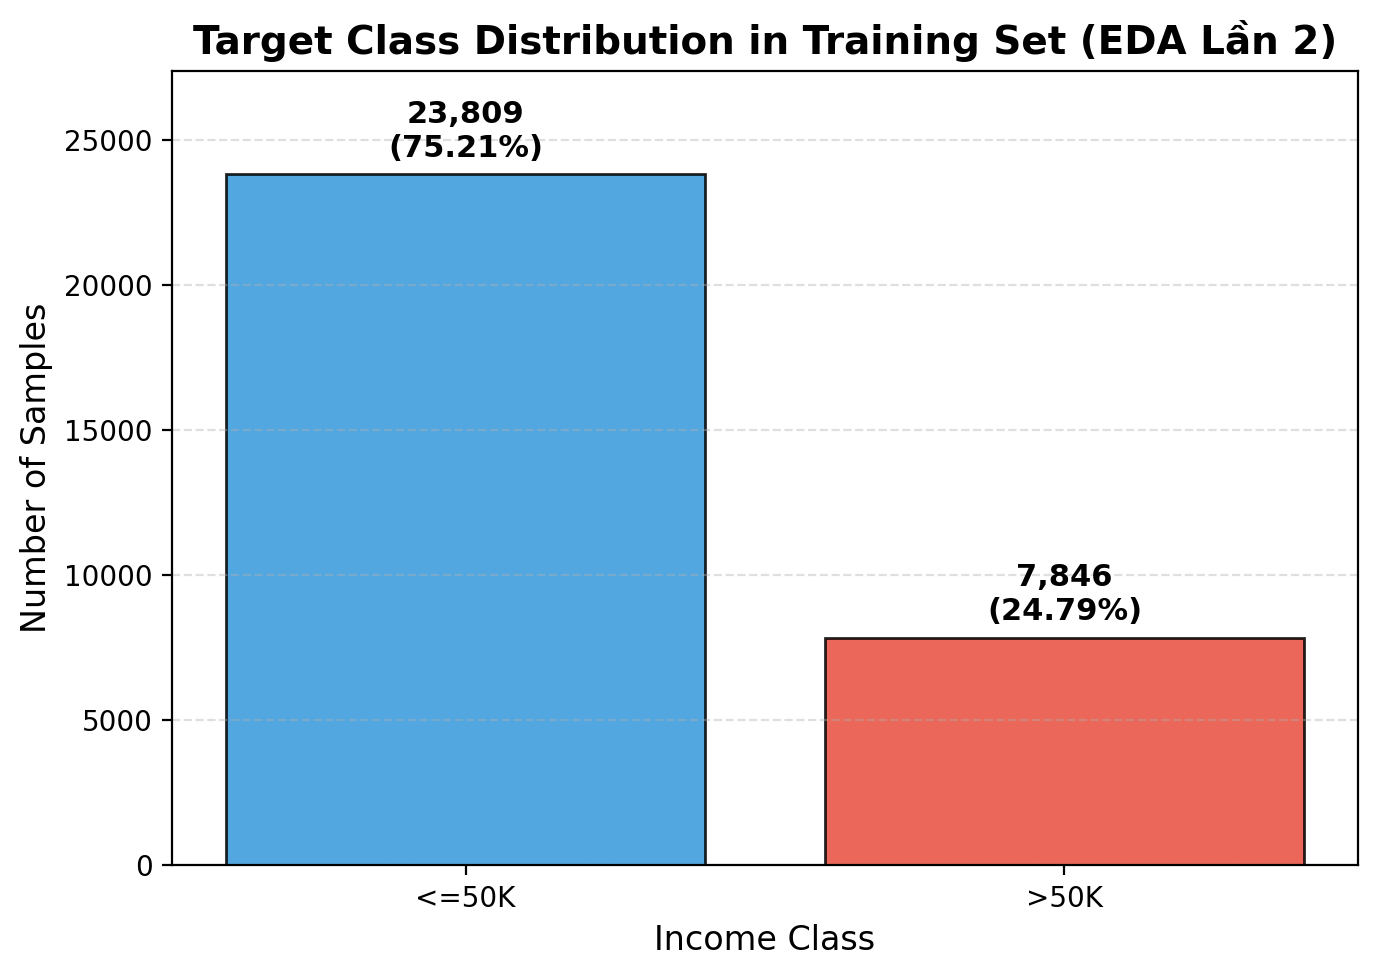
\includegraphics[width=\textwidth]{figures/tab_target_dist.png}
    \caption{Phân phối nhãn mục tiêu trên tập huấn luyện}
    \label{fig:tab_target_dist}
\end{subfigure}
\hfill
\begin{subfigure}[b]{0.48\textwidth}
    \centering
    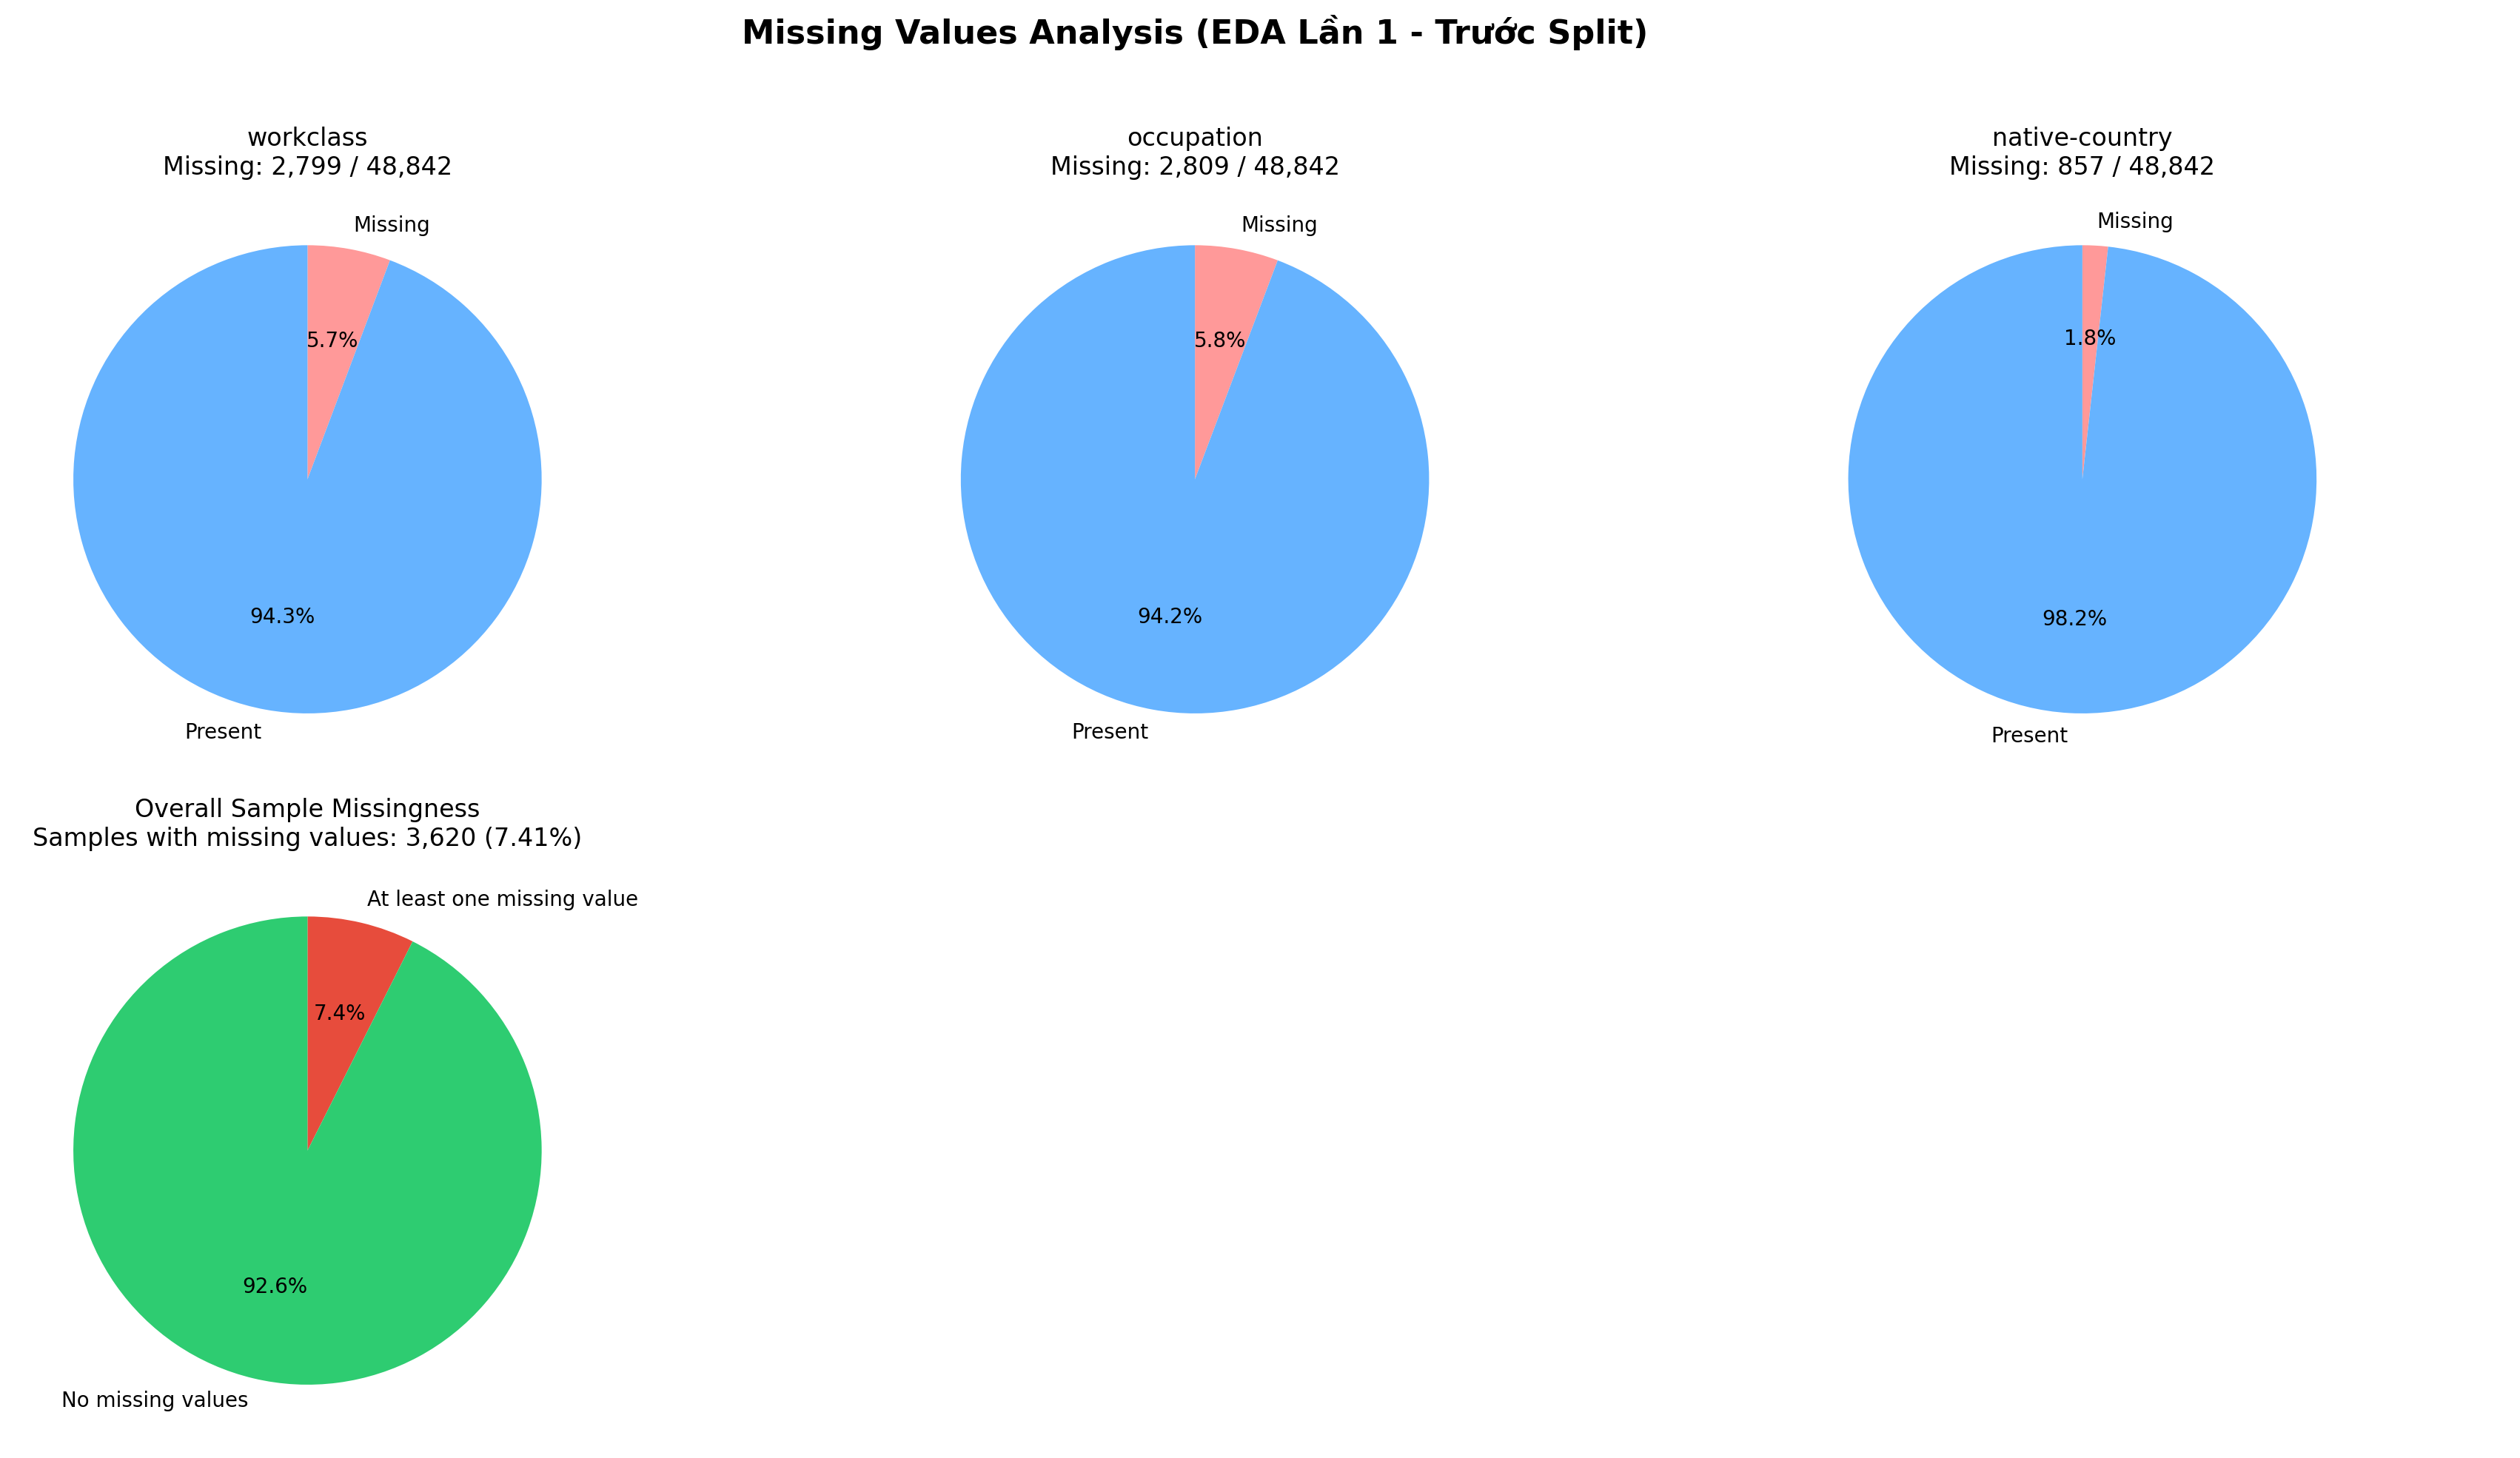
\includegraphics[width=\textwidth]{figures/tab_missing_values.png}
    \caption{Phân tích tỷ lệ giá trị thiếu (Missing Values)}
    \label{fig:tab_missing_values}
\end{subfigure}
\caption{Khảo sát phân phối nhãn và giá trị thiếu trên tập dữ liệu Adult}
\end{figure}

Qua bước khảo sát chất lượng thô (EDA Lần 1) trên toàn bộ tập dữ liệu, nhóm rút ra hai nhận định then chốt:
\begin{enumerate}
    \item \textbf{Mất cân bằng lớp (Class Imbalance):} Tập huấn luyện có 24.720 mẫu \texttt{<=50K} (chiếm 75,92\%) và 7.841 mẫu \texttt{>50K} (chiếm 24,08\%), tạo ra tỷ lệ mất cân bằng $\approx 3{,}15:1$ (Hình \ref{fig:tab_target_dist}). Do đó, độ đo Accuracy đơn thuần sẽ bị lệch; cần theo dõi chặt chẽ Macro-F1, Precision, Recall và ROC-AUC cho lớp thiểu số \texttt{>50K}.
    \item \textbf{Giá trị thiếu (Missing Values):} Dữ liệu thô sử dụng ký tự \texttt{?} để biểu diễn ô trống trong 3 biến phân loại: \texttt{workclass} (1.836 mẫu thiếu, 5,64\%), \texttt{occupation} (1.843 mẫu thiếu, 5,66\%) và \texttt{native-country} (583 mẫu thiếu, 1,79\%) (Hình \ref{fig:tab_missing_values}). Các giá trị thiếu này được điền bằng giá trị xuất hiện nhiều nhất (Mode Imputation) được fit hoàn toàn trên tập train.
\end{enumerate}

\subsection{Chuẩn bị dữ liệu và Lựa chọn Đặc trưng (EDA Lần 2 \& Preprocessing)}
Quy trình tiền xử lý tuân thủ nghiêm ngặt nguyên tắc \textit{No Data Leakage}: mọi phép biến đổi, chọn lọc đặc trưng và thống kê chuẩn hóa đều chỉ được fit trên tập huấn luyện, sau đó áp dụng biến đổi tất định lên tập validation và test.

\begin{figure}[H]
\centering
\begin{subfigure}[b]{0.48\textwidth}
    \centering
    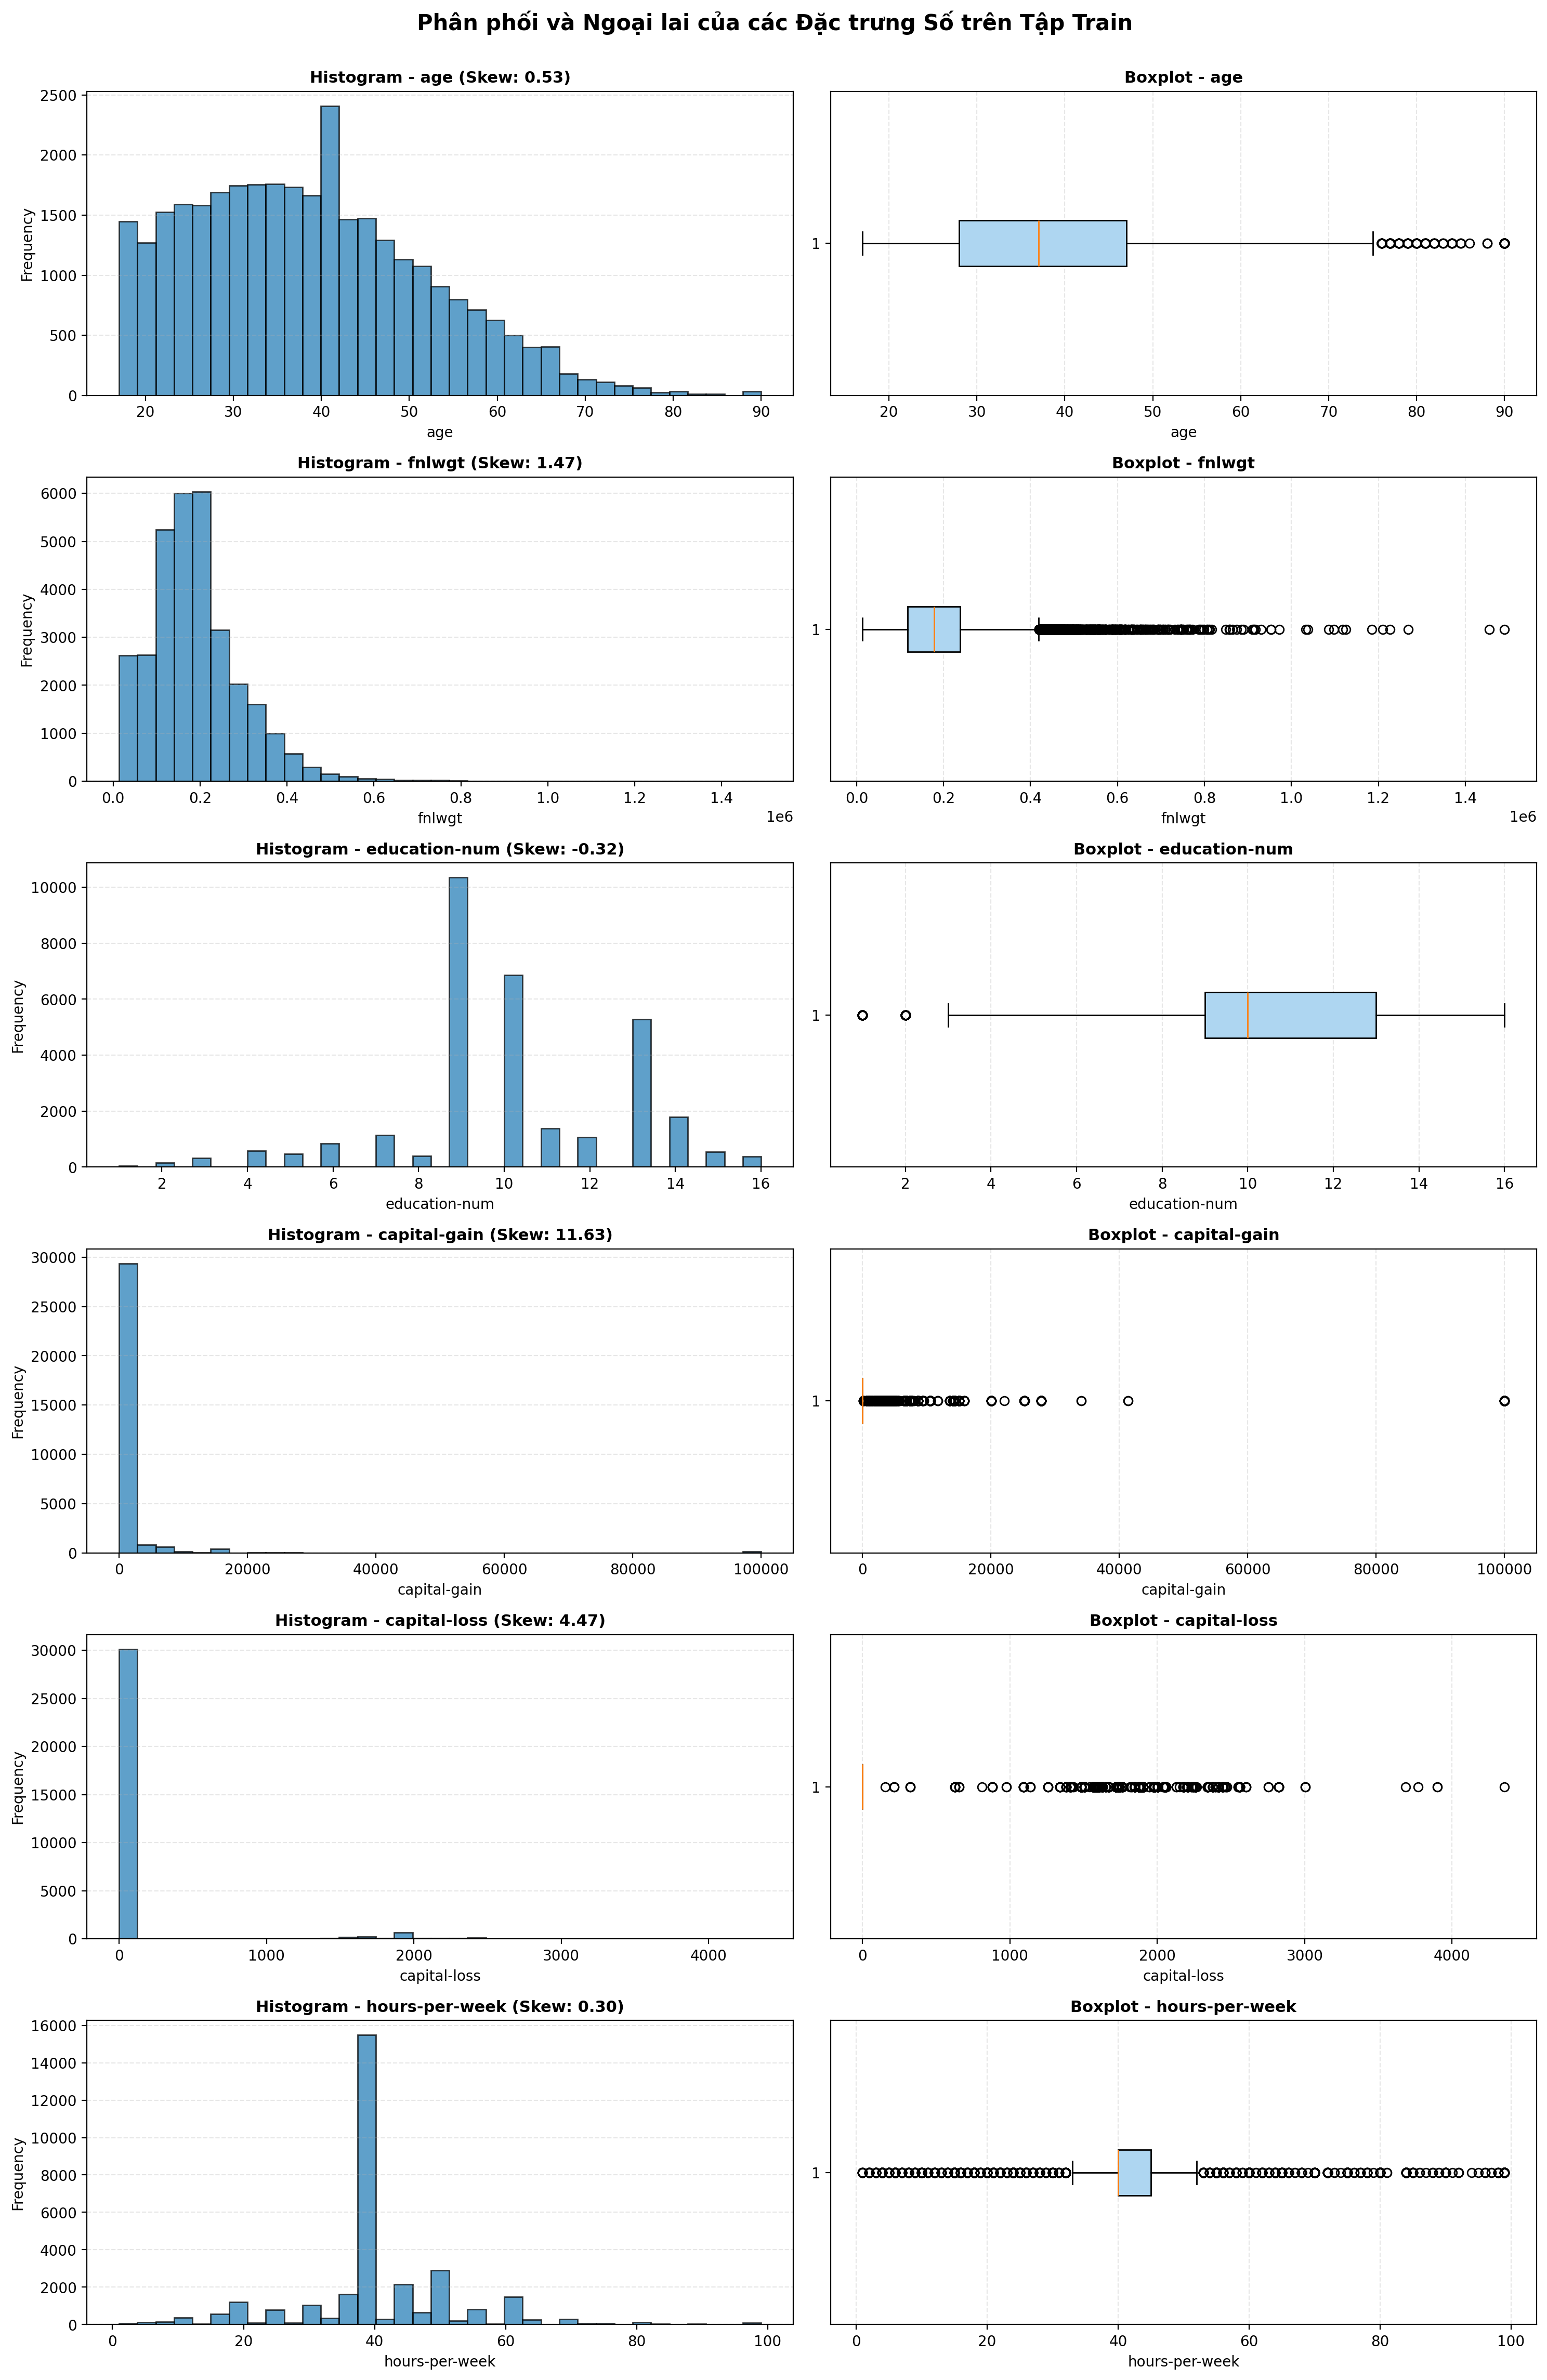
\includegraphics[width=\textwidth]{figures/tab_numerical_dist.png}
    \caption{Phân phối các đặc trưng số}
    \label{fig:tab_num_dist}
\end{subfigure}
\hfill
\begin{subfigure}[b]{0.48\textwidth}
    \centering
    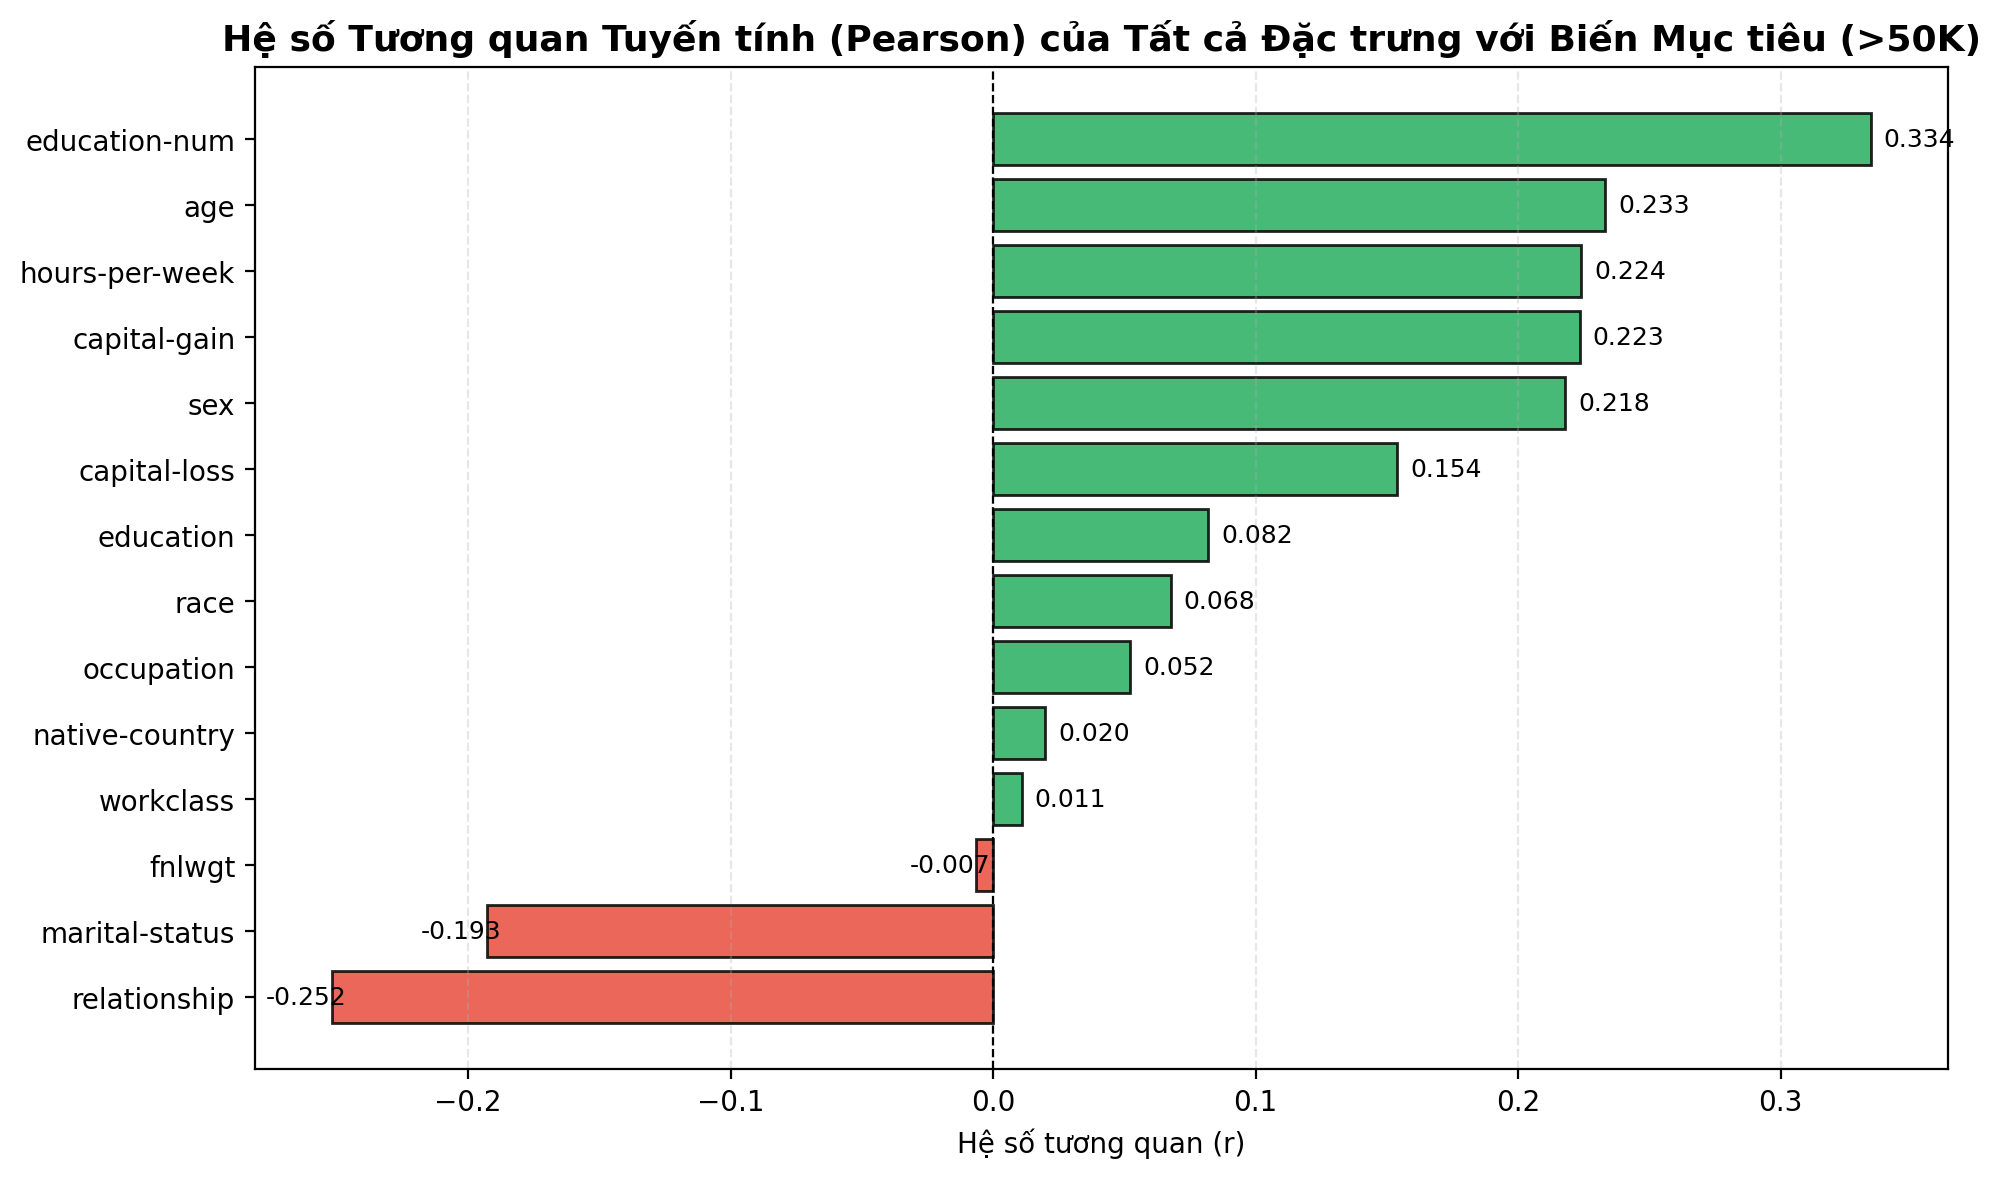
\includegraphics[width=\textwidth]{figures/tab_feature_corr.png}
    \caption{Tương quan tuyến tính với biến mục tiêu}
    \label{fig:tab_corr}
\end{subfigure}
\caption{Khảo sát phân phối đặc trưng số và mức độ tương quan}
\end{figure}

\begin{figure}[H]
\centering
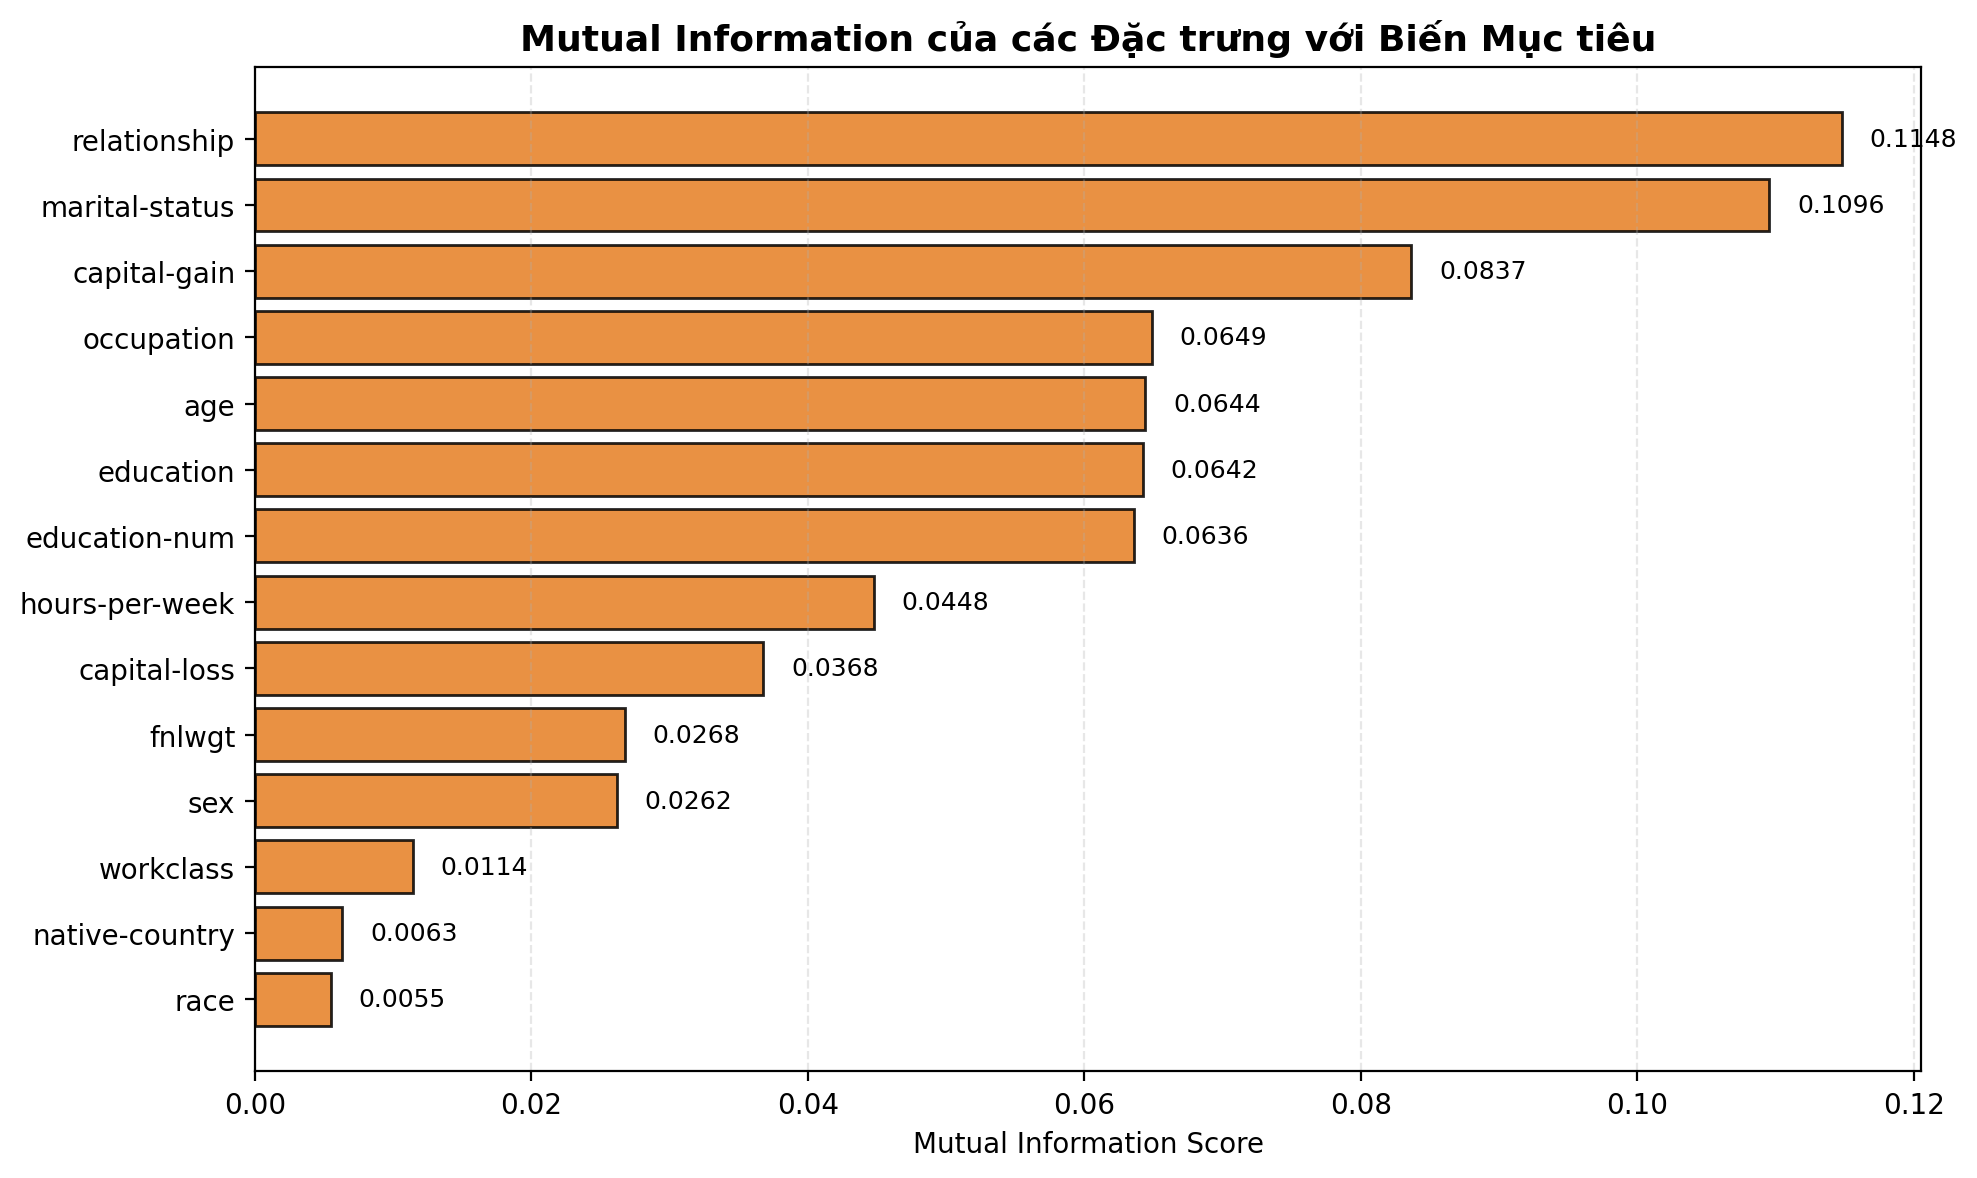
\includegraphics[width=0.7\textwidth]{figures/tab_feature_importance.png}
\caption{Điểm thông tin tương hỗ (Mutual Information Score) của các đặc trưng với biến mục tiêu}
\label{fig:tab_mi}
\end{figure}

Dựa trên kết quả đối chiếu giữa ma trận tương quan Pearson và điểm thông tin tương hỗ Mutual Information (Hình \ref{fig:tab_corr} và \ref{fig:tab_mi}):
\begin{itemize}
    \item \textbf{Loại bỏ thuộc tính dư thừa:} Thuộc tính \texttt{education} và \texttt{education-num} có quan hệ song ánh $1-1$ hoàn hảo (ví dụ: \texttt{Bachelors} $\leftrightarrow 13$, \texttt{HS-grad} $\leftrightarrow 9$). Để triệt tiêu hoàn toàn hiện tượng đa cộng tuyến, cột danh mục \texttt{education} được loại bỏ, giữ lại cột số nguyên thứ bậc \texttt{education-num}.
    \item \textbf{Loại bỏ thuộc tính độ liên quan thấp:} Thuộc tính \texttt{native-country} thỏa mãn đồng thời hai tiêu chí loại bỏ định lượng: tương quan Pearson $|r| < 0{,}05$ và điểm Mutual Information $< 0{,}010$, đóng góp thông tin phân loại rất mờ nhạt nhưng lại làm bùng nổ số chiều khi One-Hot Encoding. Do đó, cột này được loại bỏ.
    \item \textbf{Mã hóa danh mục (One-Hot Encoding):} 6 biến phân loại còn lại (\texttt{workclass}, \texttt{marital-status}, \texttt{occupation}, \texttt{relationship}, \texttt{race}, \texttt{sex}) được mã hóa qua \texttt{OneHotEncoder(handle\_unknown='ignore')}, tạo ra 41 cột nhị phân dummy.
    \item \textbf{Chuẩn hóa đặc trưng số (Feature Scaling):} Các biến số có thang đo phân tán mạnh (ví dụ \texttt{capital-gain} lên đến 99.999 so với \texttt{age} chỉ từ 17--90) được chuẩn hóa bằng \texttt{StandardScaler} cho các mô hình nhạy cảm khoảng cách (KNN, SVM, MLP).
    \item \textbf{Chiến lược xử lý mất cân bằng:} Tập huấn luyện được áp dụng \texttt{RandomOverSampler} cho KNN và Gaussian Naive Bayes; với XGBoost sử dụng tham số \texttt{scale\_pos\_weight} bằng tỷ lệ mất cân bằng $\approx 3{,}15$; với SVM dùng \texttt{class\_weight}; và với MLP tích hợp \texttt{pos\_weight} trong hàm mất mát \texttt{BCEWithLogitsLoss}.
\end{itemize}

\subsection{Phân tích và Mô hình hóa}
Nghiên cứu tiến hành huấn luyện và so sánh đồng thời năm thuật toán học máy đại diện cho các trường phái khác nhau:
\begin{enumerate}
    \item \textbf{K-Nearest Neighbors (KNN):} $k=5$, đo khoảng cách Euclidean trên không gian đặc trưng đã chuẩn hóa z-score và cân bằng lớp bằng oversampling.
    \item \textbf{Gaussian Naive Bayes:} Mô hình xác suất dựa trên định lý Bayes, huấn luyện trên tập dữ liệu one-hot đã oversampling.
    \item \textbf{Support Vector Machine (SVM):} Sử dụng RBF kernel phi tuyến, tích hợp \texttt{class\_weight} để bù trừ tổn thất cho lớp thiểu số.
    \item \textbf{Multi-Layer Perceptron (MLP):} Mạng nơ-ron sâu với kiến trúc Fully Connected $(47 \to 128 \to 64 \to 32 \to 1)$, hàm kích hoạt ReLU, Dropout tỷ lệ 0.3, tối ưu bằng Adam kết hợp kỹ thuật Early Stopping (patience=10).
    \item \textbf{XGBoost:} Thuật toán Gradient Boosted Decision Trees với 200 estimators, độ sâu cây $max\_depth=6$, $learning\_rate=0{,}05$ và $scale\_pos\_weight=3{,}15$.
\end{enumerate}

\begin{figure}[H]
\centering
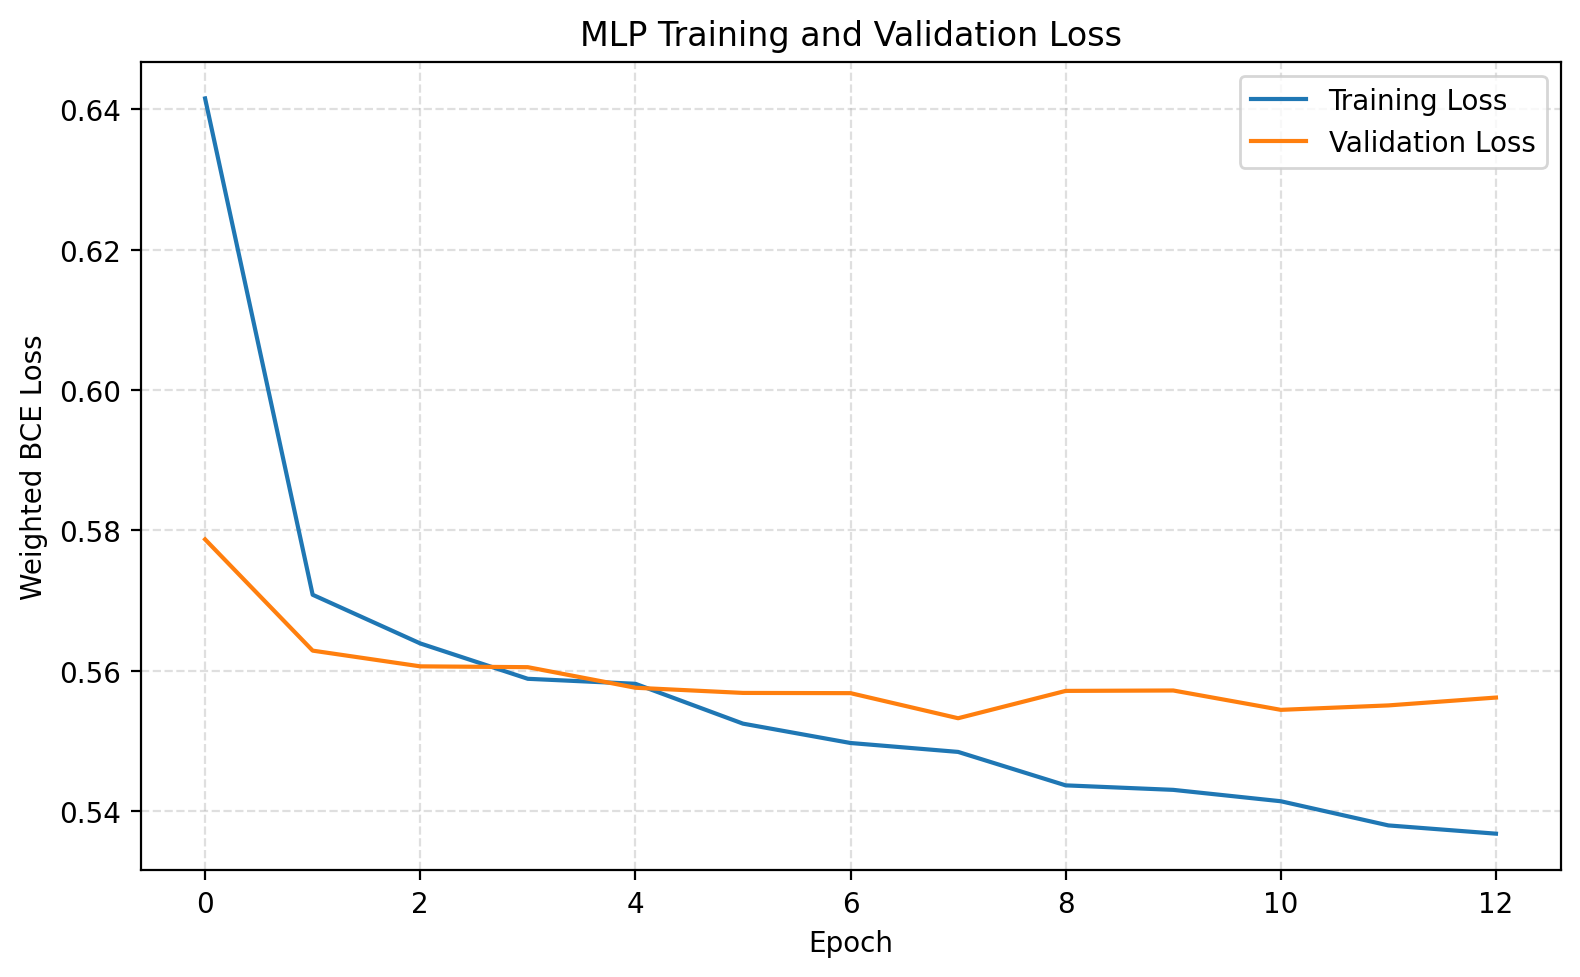
\includegraphics[width=0.65\textwidth]{figures/tab_mlp_curves.png}
\caption{Đường cong huấn luyện (Loss và ROC-AUC) của mô hình mạng nơ-ron MLP}
\label{fig:tab_mlp_curves}
\end{figure}

\begin{table}[H]
\centering
\caption{Bảng kết quả đánh giá đối chuẩn các mô hình trên tập kiểm thử độc lập (Test Set)}
\label{tab:tabular_results}
\small
\begin{tabular}{lrrrrr}
\toprule
\textbf{Thuật toán} & \textbf{Accuracy} & \textbf{Precision (>50K)} & \textbf{Recall (>50K)} & \textbf{F1-Score (>50K)} & \textbf{ROC-AUC} \\
\midrule
\textbf{XGBoost}     & \textbf{83{,}36\%} & \textbf{61{,}64\%} & 86{,}97\% & \textbf{0{,}7214} & \textbf{0{,}9267} \\
MLP (PyTorch)        & 80{,}91\% & 57{,}60\% & 86{,}97\% & 0{,}6931 & 0{,}9095 \\
SVM (RBF Kernel)     & 80{,}29\% & 56{,}65\% & \textbf{87{,}21\%} & 0{,}6868 & 0{,}8987 \\
KNN ($k=5$)          & 78{,}36\% & 54{,}50\% & 76{,}80\% & 0{,}6375 & 0{,}8571 \\
Gaussian Naive Bayes & 78{,}24\% & 62{,}96\% & 29{,}63\% & 0{,}4029 & 0{,}8280 \\
\bottomrule
\end{tabular}
\end{table}

\begin{figure}[H]
\centering
\begin{subfigure}[b]{0.48\textwidth}
    \centering
    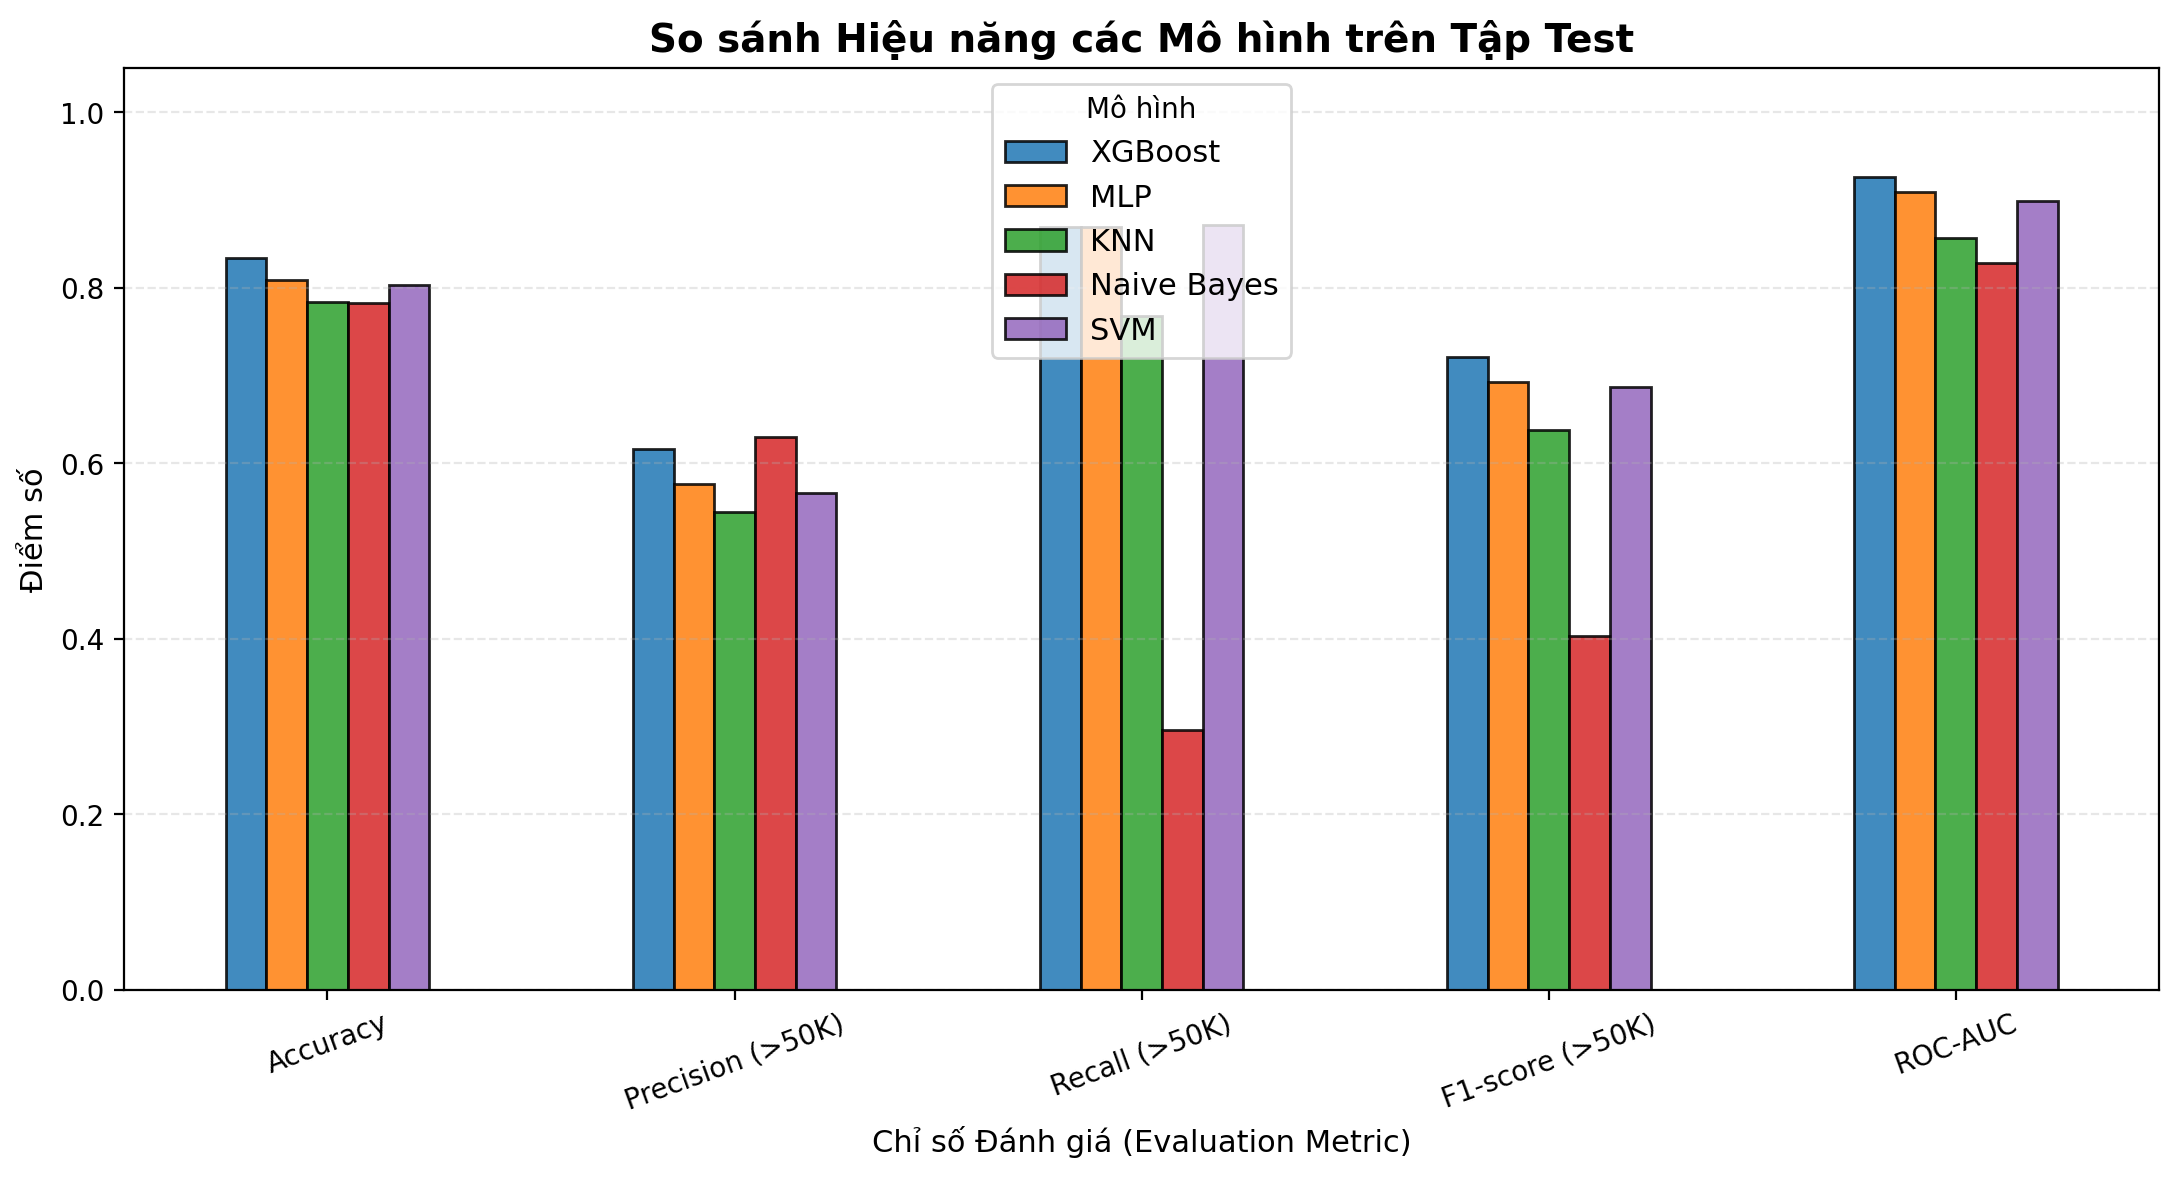
\includegraphics[width=\textwidth]{figures/tab_metrics_comparison.png}
    \caption{Biểu đồ so sánh các chỉ số đo lường chính}
    \label{fig:tab_metrics}
\end{subfigure}
\hfill
\begin{subfigure}[b]{0.48\textwidth}
    \centering
    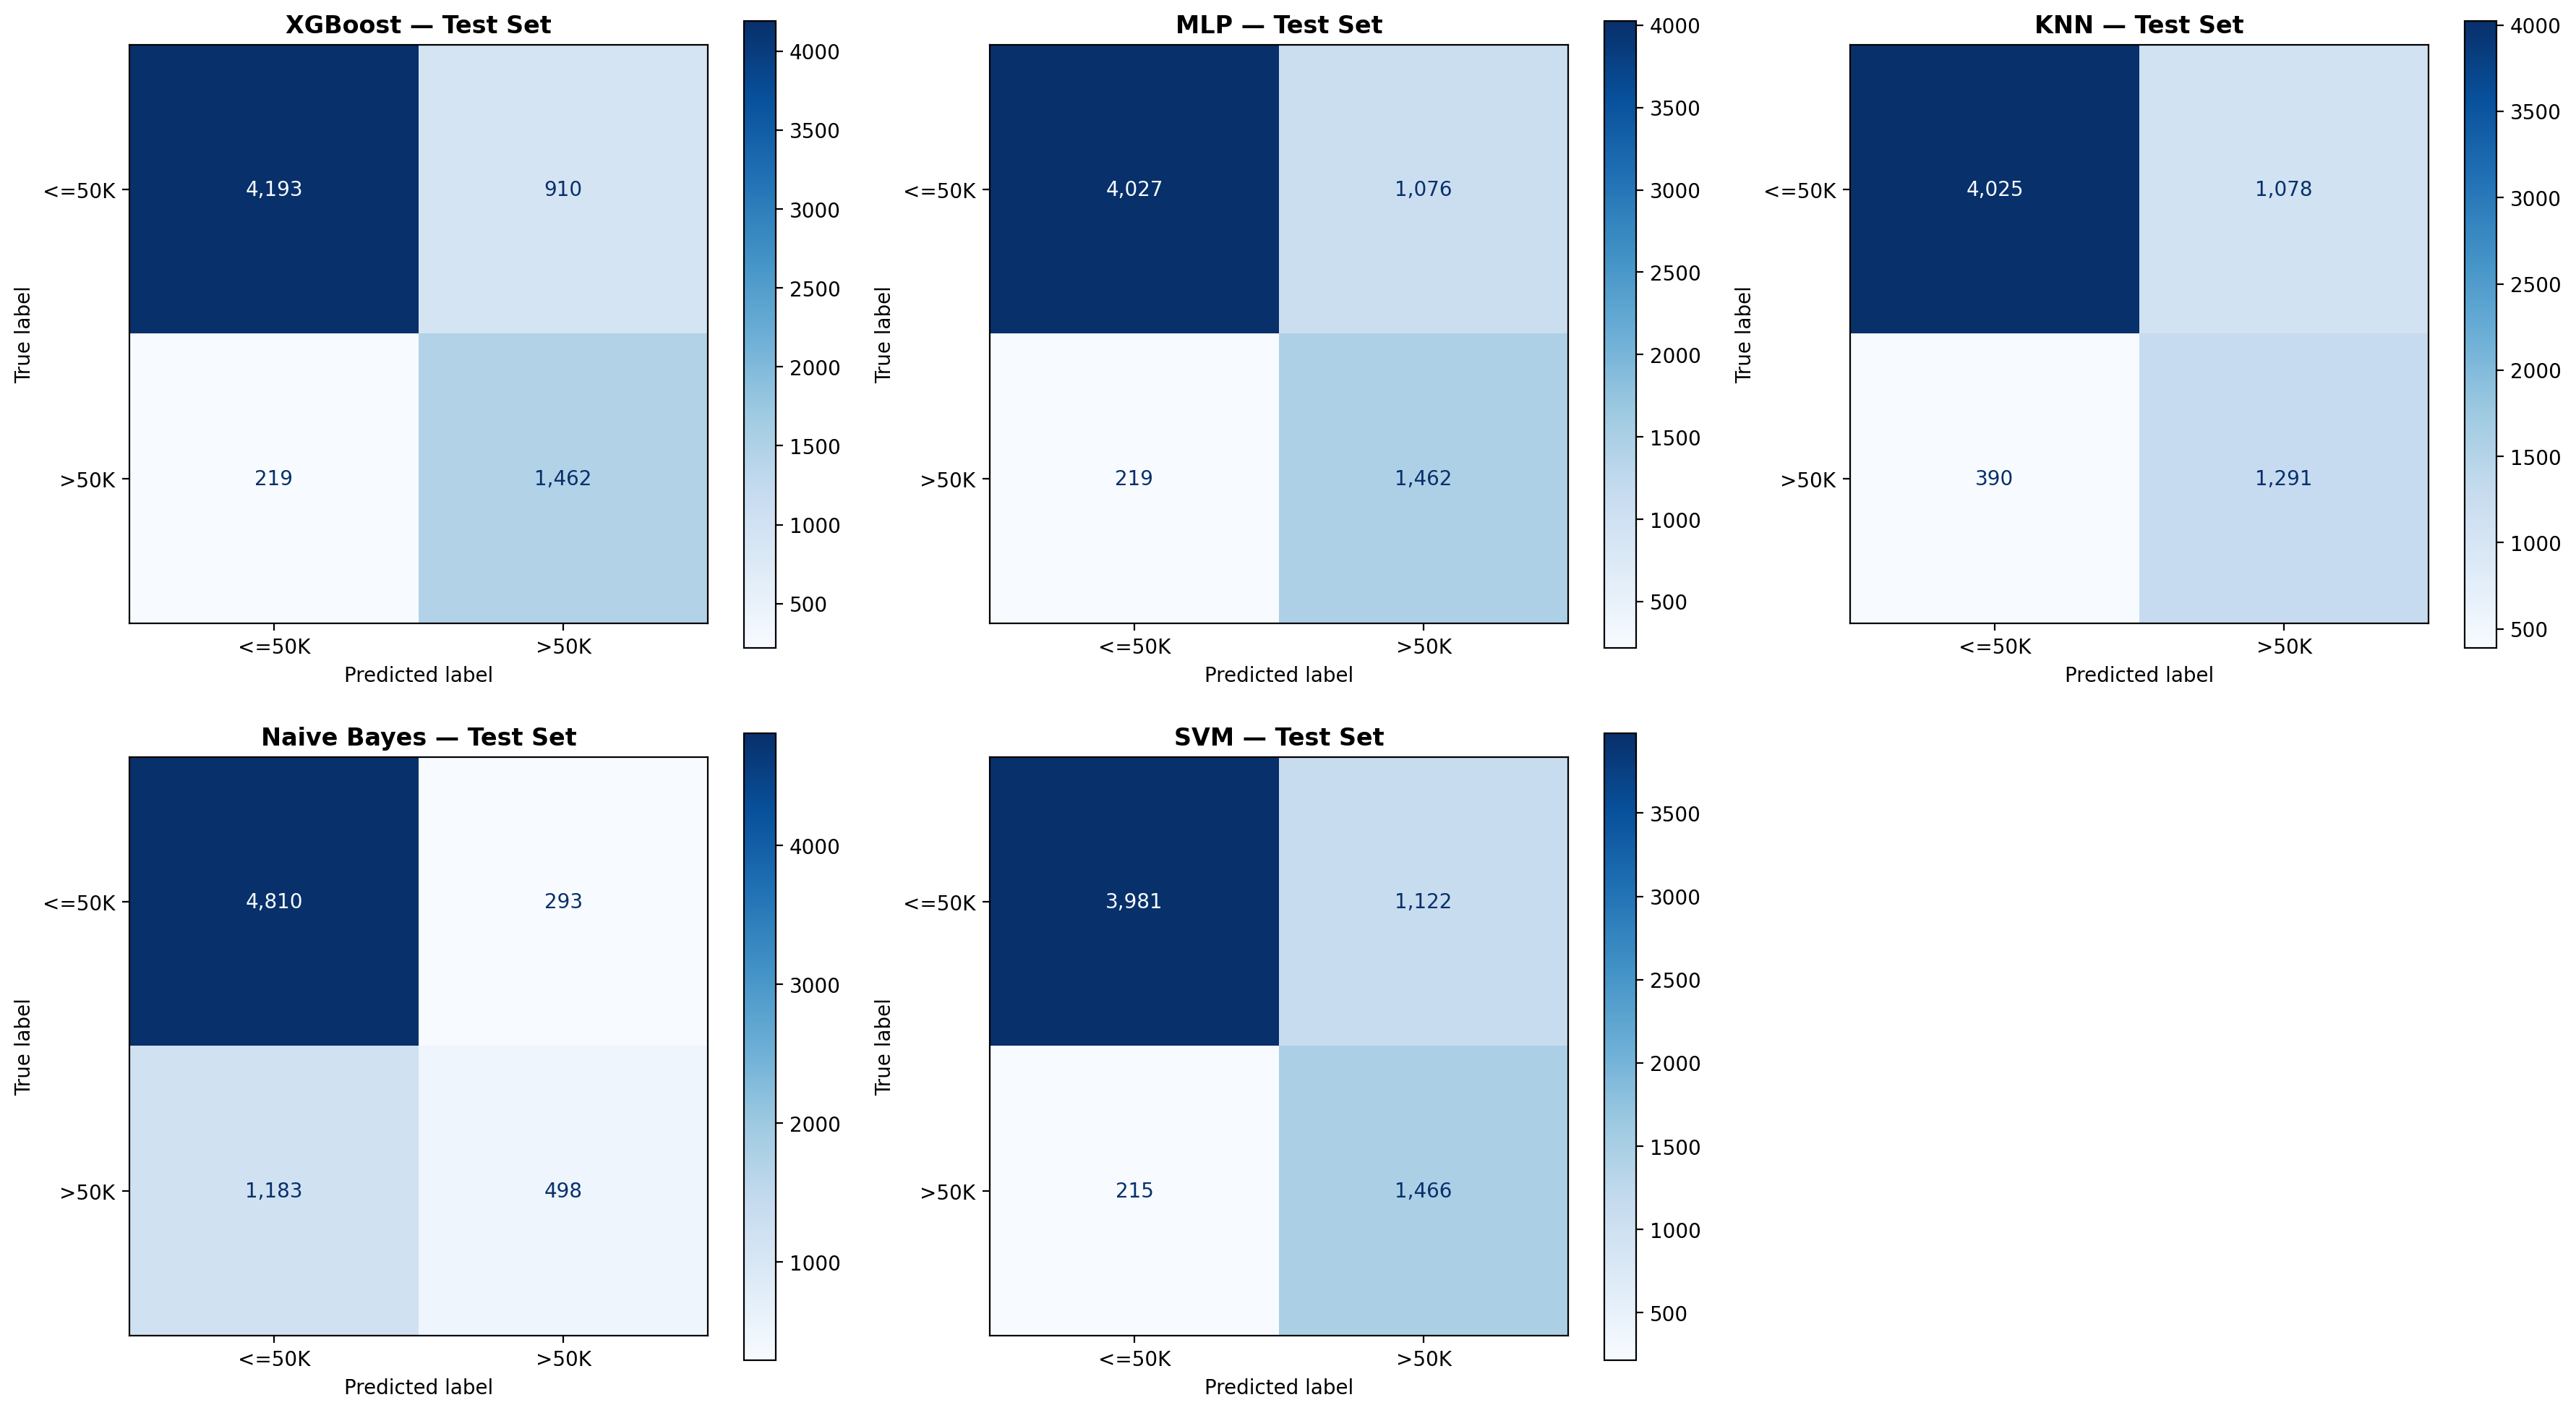
\includegraphics[width=\textwidth]{figures/tab_confusion_matrices.png}
    \caption{Ma trận nhầm lẫn (Confusion Matrices) trên Test Set}
    \label{fig:tab_cm}
\end{subfigure}
\caption{So sánh trực quan hiệu năng và ma trận nhầm lẫn giữa năm thuật toán}
\end{figure}

\subsection{Tổng kết và Hướng mở rộng}
Kết quả thực nghiệm trên bảng \ref{tab:tabular_results} cho thấy:
\begin{itemize}
    \item \textbf{XGBoost} là thuật toán dẫn đầu toàn diện trên bài toán Adult Census Income, đạt ROC-AUC ấn tượng $0{,}9267$, F1-score lớp thiểu số $0{,}7214$ và độ chính xác tổng thể $83{,}36\%$. Khả năng phân nhánh phi tuyến cùng cơ chế điều chuẩn gradient giúp cây quyết định nắm bắt tốt mối quan hệ phức tạp giữa các tương tác đặc trưng nhân khẩu học.
    \item \textbf{Mạng nơ-ron MLP} và \textbf{SVM} thể hiện năng lực dự báo bám sát (ROC-AUC lần lượt đạt $0{,}9095$ và $0{,}8987$), đồng thời đạt độ nhạy (Recall) rất cao đối với nhóm thu nhập cao ($\approx 87\%$).
    \item \textbf{Gaussian Naive Bayes} bộc lộ nhược điểm rõ rệt khi Recall lớp \texttt{>50K} chỉ đạt $29{,}63\%$, do giả định các biến độc lập có điều kiện bị vi phạm nghiêm trọng trên các cột phân loại One-Hot Encoding.
    \item \textbf{Hướng mở rộng:} Tích hợp các kỹ thuật sinh mẫu tổng hợp phi tuyến tiên tiến (SMOTE-NC, ADASYN) để làm mượt ranh giới phân loại; tối ưu hóa không gian siêu tham số bằng Bayesian Optimization; và ứng dụng SHAP (SHapley Additive exPlanations) để diễn giải tầm quan trọng cục bộ của từng biến đối với quyết định tín dụng/thu nhập của từng cá nhân.
\end{itemize}

% ==============================================================================
% SECTION 2: IMAGE
% ==============================================================================
\newpage
\section{Dữ liệu Ảnh (Image): Phân loại Cảnh tự nhiên Intel Image Classification}

\subsection{Mô tả tập dữ liệu và Phân tích Thám mã (EDA)}
Bài toán phân loại ảnh cảnh quan tự nhiên được thực hiện trên tập dữ liệu \textbf{Intel Image Classification} \cite{intel_dataset}, được công bố bởi Intel và lưu trữ trên Kaggle. Đây là bài toán phân loại ảnh đa lớp có giám sát gồm 6 lớp cảnh quan tự nhiên và nhân tạo:
\begin{center}
\texttt{buildings}, \texttt{forest}, \texttt{glacier}, \texttt{mountain}, \texttt{sea}, \texttt{street}
\end{center}

Tập dữ liệu thô gồm 17.034 ảnh có nhãn (thuộc hai thư mục \texttt{seg\_train} và \texttt{seg\_test}). Toàn bộ 7.301 ảnh không nhãn trong \texttt{seg\_pred} được chủ động loại bỏ khỏi nghiên cứu. Khảo sát kỹ thuật toàn diện cho thấy:
\begin{itemize}
    \item \textbf{Cân bằng nhãn tự nhiên:} Số lượng mẫu giữa 6 lớp tương đối đồng đều (dao động từ 2.689 đến 3.037 ảnh mỗi lớp, tỷ lệ $max/min \approx 1{,}14:1$, xem Hình \ref{fig:img_counts}). Do đó, hàm mất mát Cross-Entropy tiêu chuẩn là tối ưu mà không cần áp dụng oversampling làm biến dạng phân phối thực tế.
    \item \textbf{Kích thước và hệ màu:} 100\% ảnh đạt chuẩn định dạng 3 kênh màu RGB. Kích thước ảnh trung vị là $150 \times 150$ pixel. Không có ảnh nào bị lỗi giải mã (decode) hoặc thiếu kênh màu.
    \item \textbf{Chất lượng ảnh và phân phối độ sáng:} Khảo sát phân phối độ sáng, tương phản và phương sai toán tử Laplacian (đo độ sắc nét/biên cạnh) cho thấy có 137 ảnh tối (\texttt{brightness} $< 40$) và 8 ảnh có độ tương phản rất thấp (Hình \ref{fig:img_dist}). Tuy nhiên, đây là đặc tính vật lý tự nhiên của các khung cảnh đêm hoặc bề mặt tuyết sương mù, do đó nhóm quyết định không can thiệp bộ lọc nhân tạo (như CLAHE) để bảo toàn miền đặc trưng gốc của bài toán.
\end{itemize}

\begin{figure}[H]
\centering
\begin{subfigure}[b]{0.48\textwidth}
    \centering
    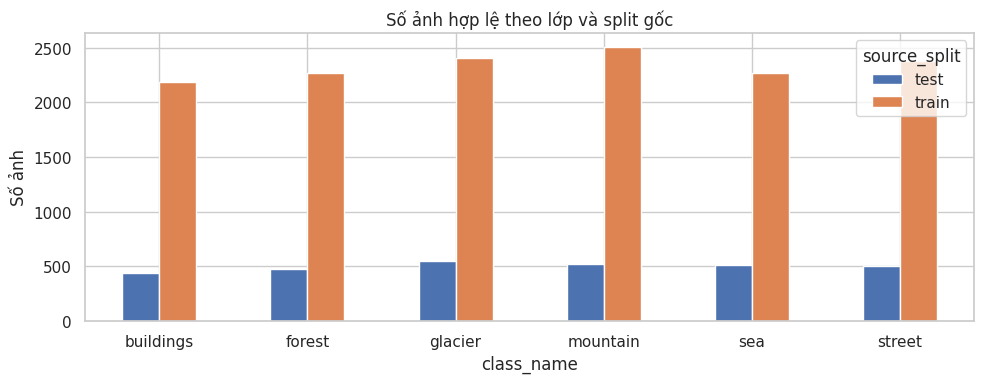
\includegraphics[width=\textwidth]{figures/img_class_counts.png}
    \caption{Phân phối số ảnh theo 6 lớp trong train và test gốc}
    \label{fig:img_counts}
\end{subfigure}
\hfill
\begin{subfigure}[b]{0.48\textwidth}
    \centering
    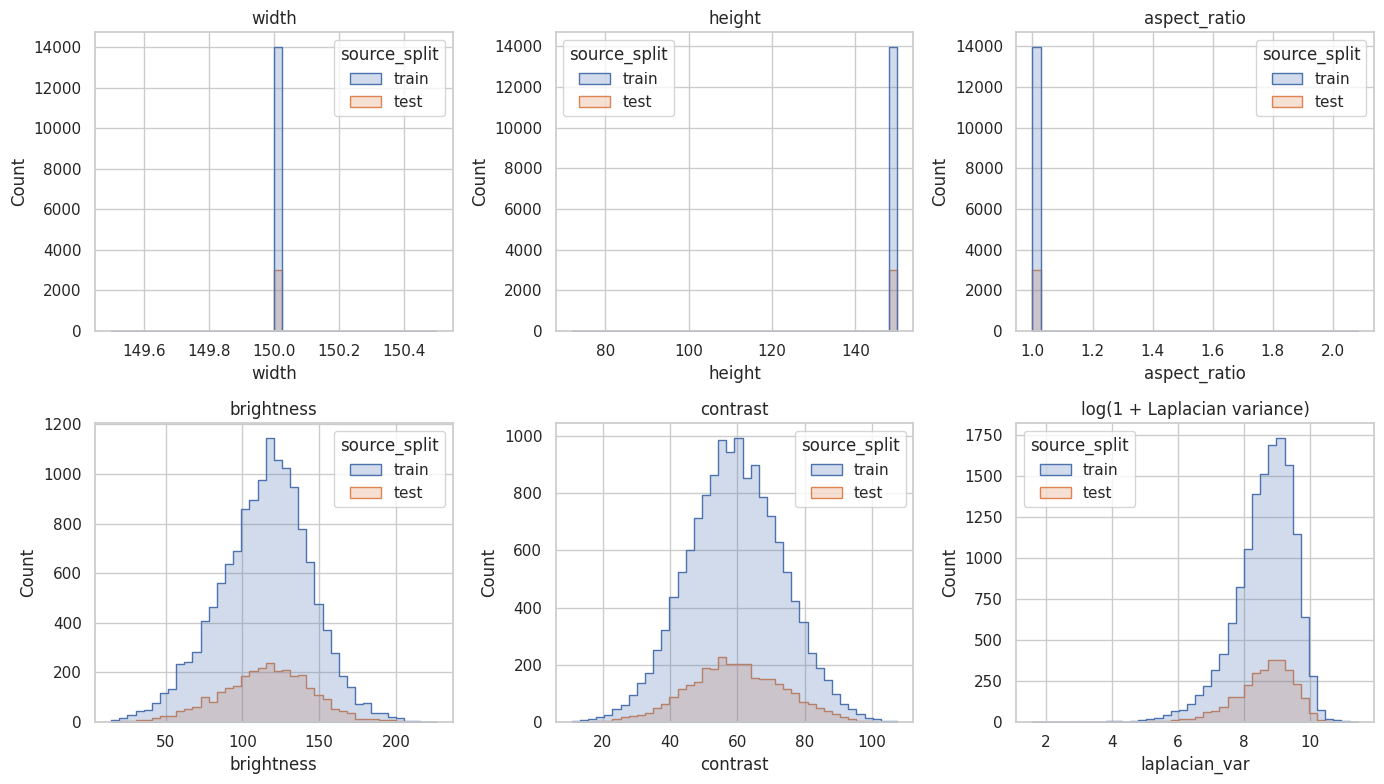
\includegraphics[width=\textwidth]{figures/img_eda_distributions.png}
    \caption{Phân phối kích thước, màu sắc và độ sắc nét Laplacian}
    \label{fig:img_dist}
\end{subfigure}
\caption{Khảo sát EDA định lượng trên tập dữ liệu Intel Image Classification}
\end{figure}

\subsection{Quy trình Làm sạch và Tiền xử lý (Data Cleaning \& Pipeline)}
\subsubsection{Khử trùng lặp và Chống rò rỉ (Deduplication)}
Để loại bỏ triệt để hiện tượng rò rỉ dữ liệu (Data Leakage) giữa các tập đánh giá, nhóm tiến hành băm dữ liệu pixel RGB (MD5 hash) trên từng bức ảnh sau khi chuẩn hóa hướng EXIF. Quá trình kiểm tra phát hiện và loại bỏ 28 ảnh train vi phạm:
\begin{itemize}
    \item 3 ảnh train bị trùng lặp chính xác với ảnh trong tập test gốc (\texttt{train\_duplicate\_of\_test}).
    \item 20 ảnh trong tập train có pixel giống hệt nhau nhưng bị gán nhãn mâu thuẫn (\texttt{train\_conflicting\_labels}).
    \item 5 ảnh bị nhân bản nội bộ trong tập train (\texttt{train\_exact\_duplicate}) -- nhóm chỉ giữ lại 1 đại diện duy nhất.
\end{itemize}
Sau bước làm sạch, tập dữ liệu còn lại đúng 17.006 ảnh hợp lệ. Nhóm áp dụng phân tầng theo nhãn (\texttt{StratifiedSplit}, seed 42) để tách 20\% tập phát triển thành tập validation. Cơ cấu phân chia cuối cùng gồm:
\begin{center}
\textbf{Train:} 11.204 ảnh \quad $\vert$ \quad \textbf{Validation:} 2.802 ảnh \quad $\vert$ \quad \textbf{Test:} 3.000 ảnh (bảo toàn nguyên vẹn split test gốc của Kaggle).
\end{center}

\subsubsection{Pipeline Biến đổi ảnh và Chuẩn hóa Đầu vào}
Nhằm tương thích với miền đặc trưng của các trọng số tiền huấn luyện ImageNet-1K, pipeline biến đổi ảnh được thiết kế độc lập theo vai trò:
\begin{itemize}
    \item \textbf{Tập huấn luyện (Training Transform -- Tăng cường dữ liệu có kiểm soát):}
    \begin{align*}
        \text{PIL Image} &\xrightarrow{\text{RandomResizedCrop}} 224 \times 224 \text{ (scale 80\%--100\%, nội suy bilinear)} \\
        &\xrightarrow{\text{RandomHorizontalFlip}} \text{Lật ngang ngẫu nhiên } (p=0{,}5) \\
        &\xrightarrow{\text{ColorJitter}} \text{Biến thiên nhẹ } (\text{bright}=0{,}15, \text{contrast}=0{,}15, \text{sat}=0{,}10, \text{hue}=0{,}02) \\
        &\xrightarrow{\text{ToTensor}} \text{Tensor } [3, 224, 224], \text{ phạm vi } [0{,}0, 1{,}0] \\
        &\xrightarrow{\text{Normalize}} \text{Z-score theo ImageNet } (\mu=[0{,}485, 0{,}456, 0{,}406], \sigma=[0{,}229, 0{,}224, 0{,}225])
    \end{align*}
    \item \textbf{Tập Validation và Test (Inference Transform -- Tất định tuyệt đối):} Tuân thủ chuẩn mực đánh giá từ Torchvision: thực hiện \texttt{Resize(256)} $\to$ \texttt{CenterCrop(224)} $\to$ \texttt{ToTensor()} $\to$ \texttt{Normalize(ImageNet)}.
\end{itemize}

\subsection{Phân tích và Mô hình hóa (Transfer Learning)}
Nhóm triển khai hai bài thực nghiệm độc lập đại diện cho hai trường phái kiến trúc thị giác máy tính tiêu biểu:
\begin{enumerate}
    \item \textbf{Mô hình A -- MobileNetV3-Small} \cite{mobilenetv3}: Mạng tích chập sâu tiết kiệm tính toán (dùng depthwise separable convolution và hard-swish), pretrained \texttt{IMAGENET1K\_V1}. Classifier được thay thế bằng tầng Linear 6 đầu ra.
    \item \textbf{Mô hình B -- Vision Transformer (ViT-B/16)} \cite{vit}: Mạng Transformer chia ảnh thành 196 patch kích thước $16 \times 16$, mã hóa vị trí và sử dụng 12 tầng multi-head self-attention, pretrained \texttt{IMAGENET1K\_V1}. Classifier \texttt{heads.head} được thay thế bằng tầng Linear 6 đầu ra.
\end{enumerate}

Cả hai mô hình được huấn luyện theo quy trình \textbf{Transfer Learning hai giai đoạn}:
\begin{itemize}
    \item \textbf{Giai đoạn 1 (Head-only):} Đóng băng toàn bộ trọng số backbone (\texttt{requires\_grad=False}), giữ các lớp BatchNorm ở chế độ \texttt{eval()} để không làm hỏng running statistics. Chỉ huấn luyện classifier trong 3 epochs với learning rate $10^{-3}$.
    \item \textbf{Giai đoạn 2 (Fine-tuning):} Mở khóa toàn bộ mô hình để thích nghi đặc trưng cảnh quan, huấn luyện tối đa 15 epochs với chiến lược Differential Learning Rate: Classifier dùng lr $= 10^{-4}$, Backbone dùng lr nhỏ hơn một bậc $= 10^{-5}$ để tránh hiện tượng \textit{catastrophic forgetting}. Tối ưu hóa bằng AdamW (weight decay $10^{-4}$), batch size 16 kết hợp gradient accumulation (2 bước, effective batch size 32). Checkpoint cuối cùng được lựa chọn dựa trên Validation Macro-F1 cao nhất.
\end{itemize}

\begin{figure}[H]
\centering
\begin{subfigure}[b]{0.48\textwidth}
    \centering
    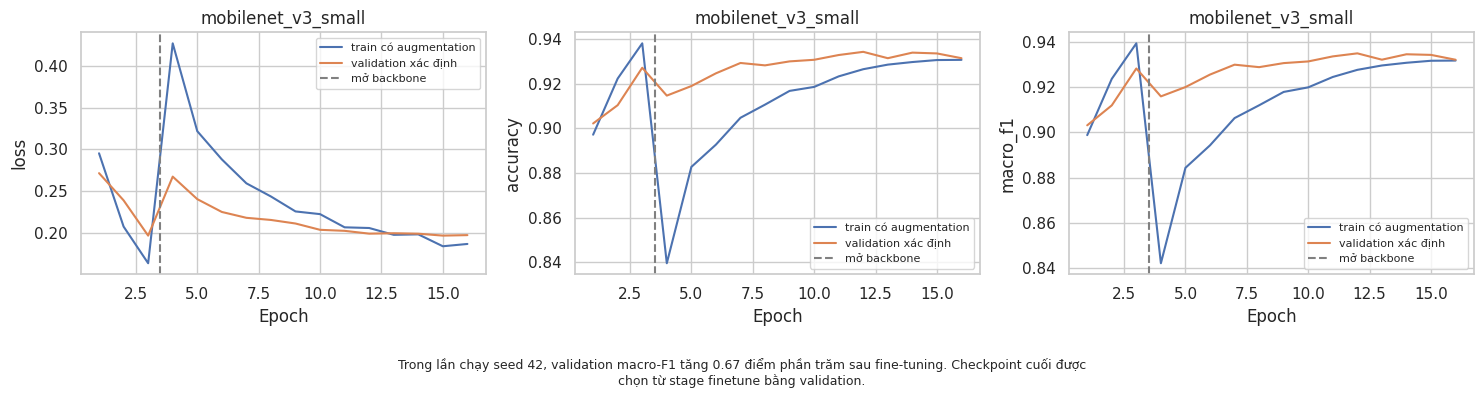
\includegraphics[width=\textwidth]{figures/img_mobilenet_curves.png}
    \caption{Learning curves của MobileNetV3-Small}
    \label{fig:img_mb_curves}
\end{subfigure}
\hfill
\begin{subfigure}[b]{0.48\textwidth}
    \centering
    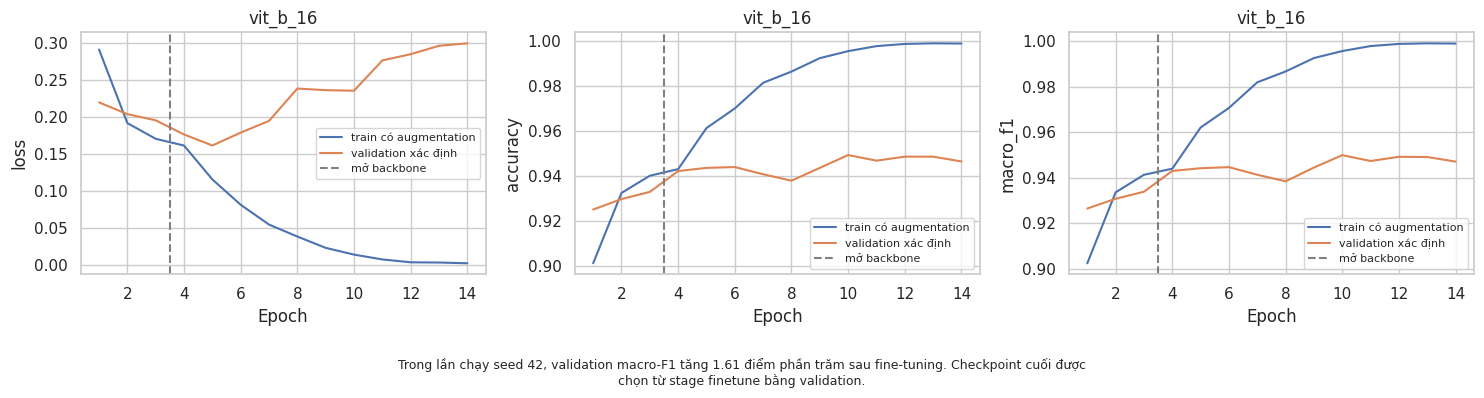
\includegraphics[width=\textwidth]{figures/img_vit_curves.png}
    \caption{Learning curves của ViT-B/16}
    \label{fig:img_vit_curves}
\end{subfigure}
\caption{Đường cong huấn luyện (Loss, Accuracy, Macro-F1) qua hai giai đoạn Transfer Learning (vạch đứt đánh dấu thời điểm mở fine-tuning)}
\end{figure}

\subsection{Tổng kết và Phân tích Lỗi (Results \& Error Analysis)}
Bảng \ref{tab:image_results} trình bày kết quả chi tiết của hai giai đoạn và đánh giá cuối cùng trên tập Test độc lập.

\begin{table}[H]
\centering
\caption{Hiệu năng thực nghiệm của MobileNetV3-Small và ViT-B/16 trên Intel Image Classification}
\label{tab:image_results}
\begin{tabular}{lrrrrr}
\toprule
\textbf{Kiến trúc mô hình} & \textbf{Head Val F1} & \textbf{FT Val F1} & \textbf{Epoch chọn} & \textbf{Test Accuracy} & \textbf{Test Macro-F1} \\
\midrule
MobileNetV3-Small & 0{,}9283 & 0{,}9350 & Epoch 9 & 92{,}43\% & 0{,}9260 \\
\textbf{ViT-B/16} & \textbf{0{,}9339} & \textbf{0{,}9500} & Epoch 7 & \textbf{94{,}50\%} & \textbf{0{,}9463} \\
\bottomrule
\end{tabular}
\end{table}

\begin{figure}[H]
\centering
\begin{subfigure}[b]{0.48\textwidth}
    \centering
    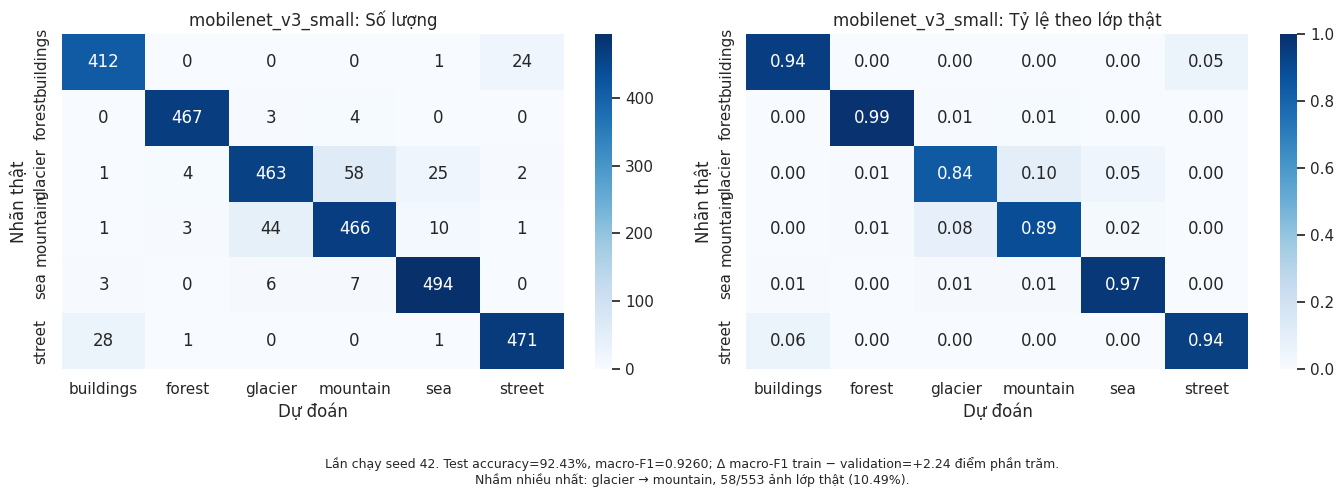
\includegraphics[width=\textwidth]{figures/img_mobilenet_confusion.png}
    \caption{Ma trận nhầm lẫn của MobileNetV3-Small}
    \label{fig:img_mb_cm}
\end{subfigure}
\hfill
\begin{subfigure}[b]{0.48\textwidth}
    \centering
    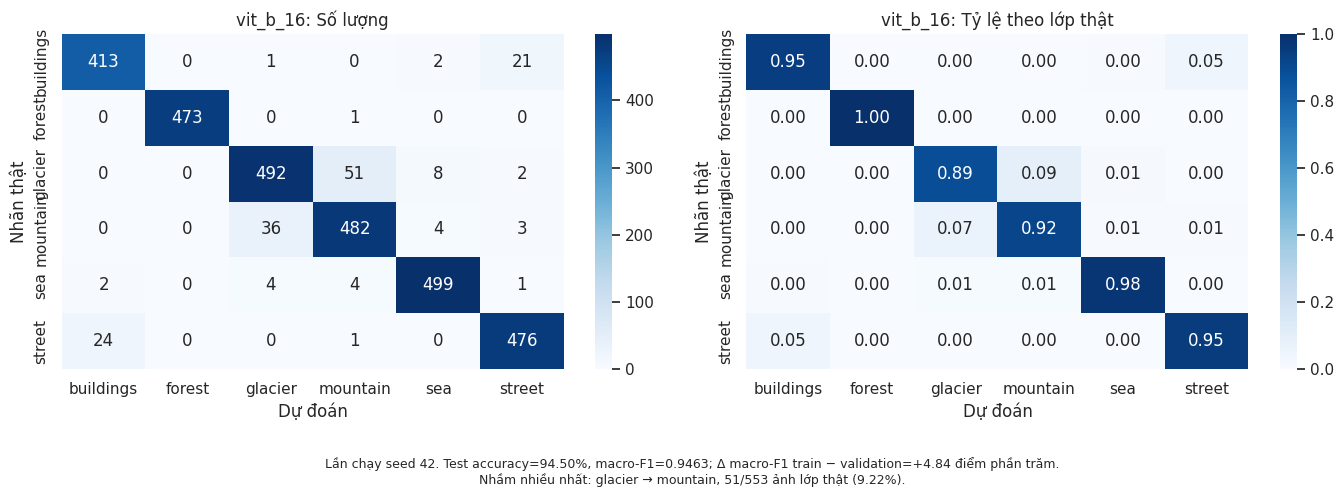
\includegraphics[width=\textwidth]{figures/img_vit_confusion.png}
    \caption{Ma trận nhầm lẫn của ViT-B/16}
    \label{fig:img_vit_cm}
\end{subfigure}
\caption{Ma trận nhầm lẫn chi tiết theo số lượng và tỷ lệ lớp thực tế trên tập kiểm thử (Test Set)}
\end{figure}

\noindent \textbf{Nhận xét và Phân tích chuyên sâu:}
\begin{itemize}
    \item \textbf{Hiệu quả của Fine-tuning:} Với cả hai mô hình, giai đoạn mở khóa backbone đều đem lại cải thiện rõ rệt cho Validation Macro-F1 (MobileNet tăng từ $0{,}9283 \to 0{,}9350$, ViT tăng từ $0{,}9339 \to 0{,}9500$). Điều này khẳng định việc tinh chỉnh nhẹ các tầng trích đặc trưng sâu giúp mạng thích nghi với các kết cấu bề mặt tự nhiên (vách đá, băng tuyết, sóng biển) tốt hơn nhiều so với việc chỉ dùng đặc trưng cố định từ ImageNet.
    \item \textbf{Sự vượt trội của Vision Transformer:} ViT-B/16 áp đảo MobileNet trên mọi tiêu chí (Test Accuracy đạt $94{,}50\%$ so với $92{,}43\%$). Cơ chế Self-Attention toàn cục cho phép mô hình thu nhận mối tương quan không gian giữa bầu trời, đỉnh núi và bề mặt nước trên toàn bức ảnh, điều mà các receptive field cục bộ của CNN khó bao quát đầy đủ.
    \item \textbf{Phân tích mẫu lỗi điển hình:} Quan sát ma trận nhầm lẫn (Hình \ref{fig:img_mb_cm} và \ref{fig:img_vit_cm}) chỉ ra lỗi sai phổ biến và mang tính hệ thống nhất của cả hai mô hình nằm ở cặp nhãn \texttt{glacier} $\leftrightarrow$ \texttt{mountain} (MobileNet nhầm 58 mẫu glacier thành mountain; ViT nhầm 51 mẫu). Nguyên nhân bản chất xuất phát từ tính đa nghĩa thị giác (Visual Ambiguity): nhiều bức ảnh núi đá bị tuyết phủ một phần hoặc sông băng nằm xen giữa các dãy núi có ranh giới phân loại rất mờ nhạt ngay cả với quan sát của con người.
\end{itemize}

% ==============================================================================
% SECTION 3: TEXT
% ==============================================================================
\newpage
\section{Dữ liệu Văn bản (Text): Phân tích Cảm xúc Tiếng Việt VLSP 2016}

\subsection{Mô tả tập dữ liệu và Phân tích Thám mã (EDA)}
Bài toán phân tích quan điểm và cảm xúc văn bản tiếng Việt (Vietnamese Sentiment Analysis) được thực hiện trên tập dữ liệu chuẩn \textbf{VLSP 2016 Shared Task} \cite{vlsp2016}. Dữ liệu bao gồm các câu bình luận, đánh giá thực tế thu thập từ mạng xã hội và các sàn thương mại điện tử tại Việt Nam.

Nhiệm vụ là bài toán phân loại văn bản đa lớp (3 lớp):
\begin{center}
\texttt{Negative} (Tiêu cực -- nhãn gốc $-1 \to 0$), \quad \texttt{Neutral} (Trung lập -- nhãn gốc $0 \to 1$), \quad \texttt{Positive} (Tích cực -- nhãn gốc $+1 \to 2$)
\end{center}

Nghiên cứu thiết lập một khung đối chứng kiểm soát nghiêm ngặt với \textbf{hai cấu hình dữ liệu phát triển} và một tập kiểm thử độc lập duy nhất:
\begin{itemize}
    \item \textbf{Tập phát triển gốc (Base Dataset):} 5.100 mẫu huấn luyện gốc phân bố cân bằng tuyệt đối (đúng 1.700 mẫu mỗi lớp, chiếm 33,33\%).
    \item \textbf{Tập phát triển tăng cường (Augmented Dataset):} 10.200 mẫu (gồm bản gốc và bản dịch vòng Back-translation Anh -- Việt, phân bố cân bằng đúng 3.400 mẫu mỗi lớp).
    \item \textbf{Tập kiểm thử độc lập (Held-out Test Dataset):} Đúng 1.050 mẫu (cân bằng hoàn hảo 350 mẫu mỗi lớp), tuyệt đối không tham gia vào quá trình huấn luyện hay sinh dữ liệu tăng cường, làm thước đo khách quan chung cho toàn bộ 12 thực nghiệm (Hình \ref{fig:txt_counts}).
\end{itemize}

\begin{figure}[H]
\centering
\begin{subfigure}[b]{0.48\textwidth}
    \centering
    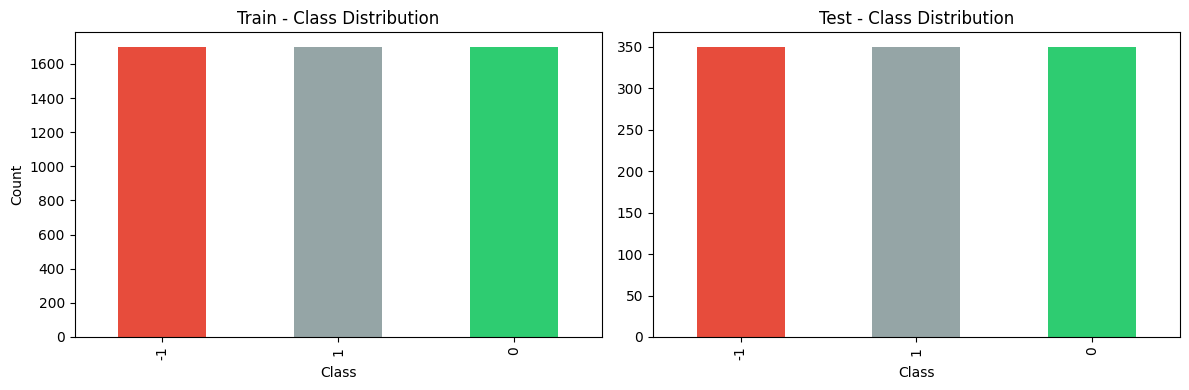
\includegraphics[width=\textwidth]{figures/txt_class_counts.png}
    \caption{Phân phối số lượng mẫu theo 3 lớp nhãn trong train và test}
    \label{fig:txt_counts}
\end{subfigure}
\hfill
\begin{subfigure}[b]{0.48\textwidth}
    \centering
    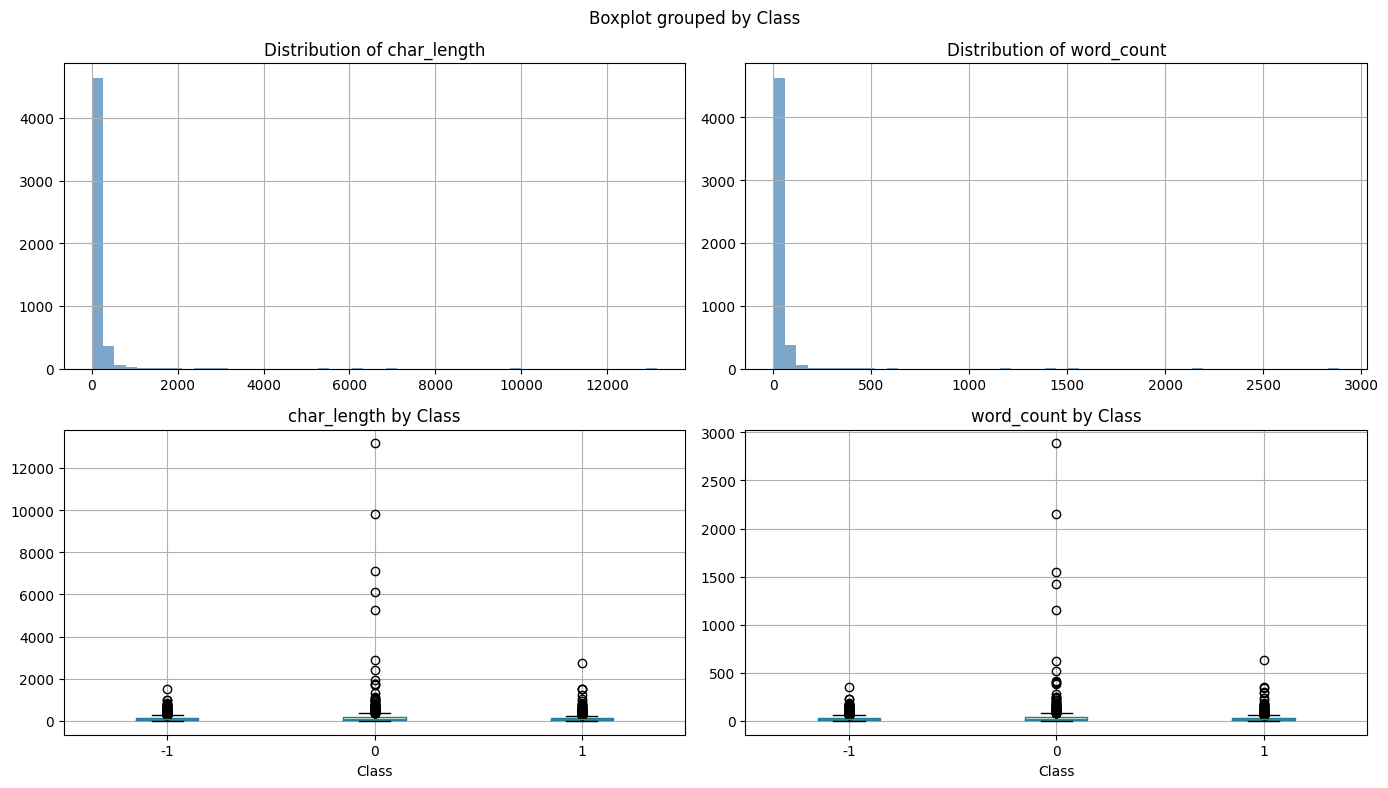
\includegraphics[width=\textwidth]{figures/txt_text_lengths.png}
    \caption{Phân phối độ dài văn bản (ký tự và từ)}
    \label{fig:txt_lengths}
\end{subfigure}
\caption{Khảo sát EDA định lượng phân phối nhãn và độ dài văn bản trên tập dữ liệu VLSP 2016}
\end{figure}

\subsection{Chuẩn bị dữ liệu và Ba Nhánh Biểu diễn Đầu vào}
Dựa trên kết quả khám phá dữ liệu (EDA), nhóm rút ra các quyết định kỹ thuật then chốt:
\begin{enumerate}
    \item \textbf{Quy chuẩn Teencode và Từ viết tắt:} Dữ liệu mạng xã hội chứa mật độ rất cao các biến thể viết tắt (*ko, đc, sp, wa, thik, mik, bthg...*). Nhóm xây dựng từ điển quy chuẩn hơn 30 cụm từ về dạng tiếng Việt chuẩn trước khi tách từ.
    \item \textbf{Ánh xạ Ký tự Cảm xúc (Emoticons):} Các biểu tượng cảm xúc phổ biến (\texttt{:)}, \texttt{:((}, \texttt{:D}, \texttt{\textasciicircum\textasciicircum}, \texttt{t.t}) được ánh xạ tường minh thành từ ngữ biểu cảm tiếng Việt (*cười, buồn, khóc, vui*) trước khi loại bỏ dấu câu đặc biệt.
    \item \textbf{Thiết lập ngưỡng chiều dài chuỗi:} Phân tích phân phối độ dài (Hình \ref{fig:txt_lengths}) cho thấy $>99\%$ câu có độ dài dưới 250 từ. Nhóm thiết lập \texttt{MAX\_SEQUENCE\_LENGTH = 300} cho nhánh Word2Vec và \texttt{max\_length = 256} cho nhánh PhoBERT, vừa bao quát ngữ cảnh vừa tối ưu hóa bộ nhớ GPU.
\end{enumerate}

Dữ liệu sau làm sạch được chuyển tiếp sang \textbf{ba nhánh biểu diễn đầu vào độc lập}:
\begin{itemize}
    \item \textbf{Nhánh 1 -- N-gram TF-IDF:} Trích xuất đặc trưng từ đơn và từ ghép (unigram + bigram) với giới hạn $max\_features = 5.000$, chuẩn hóa L2 norm.
    \item \textbf{Nhánh 2 -- Không gian vector Word2Vec CBOW 400 chiều:} Sử dụng thư viện \texttt{pyvi} để phân đoạn từ ghép tiếng Việt (ví dụ: \textit{chất lượng} $\to$ \texttt{chất\_lượng}). Các từ được ánh xạ vào ma trận trọng số embedding 400 chiều được huấn luyện trước trên kho ngữ liệu báo chí tiếng Việt (\texttt{vi-model-CBOW.bin}), giới hạn từ điển $20.000$ từ và cho phép fine-tune trong quá trình huấn luyện.
    \item \textbf{Nhánh 3 -- Subword BPE PhoBERT:} Sử dụng bộ Tokenizer chuẩn BPE của mô hình \texttt{vinai/phobert-base-v2}, tự động xử lý các token ghép dấu gạch dưới và thêm các token đặc biệt \texttt{<s>}, \texttt{</s>}, \texttt{<pad>}.
\end{itemize}

\subsection{Phân tích và Mô hình hóa (Benchmark 6 Kiến trúc)}
Nghiên cứu triển khai đồng thời sáu kiến trúc mô hình đại diện cho ba thế hệ xử lý ngôn ngữ tự nhiên:
\begin{enumerate}
    \item \textbf{TF-IDF + LinearSVC:} Mô hình phân loại Support Vector Classifier tuyến tính cổ điển, tối ưu hóa lề cực đại với tham số phạt $C=1{,}0$ và hàm mất mát Squared Hinge Loss.
    \item \textbf{TF-IDF + 1D-CNN:} Mạng tích chập 1 chiều hoạt động trên vector TF-IDF dày đặc: $\text{Dense}(1, 5000) \to \text{Conv1d}(1, 64, k=5) \to \text{ReLU} \to \text{MaxPool1d}(2) \to \text{Conv1d}(64, 128, k=5) \to \text{AdaptiveAvgPool1d}(1) \to \text{Dropout}(0{,}5) \to \text{Linear}(128, 3)$. Tối ưu bằng Adam ($lr=10^{-3}$, 15 epochs).
    \item \textbf{TextCNN} \cite{textcnn}: Kiến trúc tích chập học sâu kinh điển cho phân loại câu: ma trận Embedding trainable 400 chiều $\to$ 3 bộ lọc Conv1d song song với kích thước kernel 3, 4, 5 (mỗi nhánh 100 filters) $\to$ ReLU $\to$ Global Max Pooling $\to$ Dropout(0.5) $\to$ Linear(300, 3).
    \item \textbf{BiLSTM:} Mạng hồi quy hai chiều học biểu diễn ngữ cảnh xuôi và ngược: ma trận Embedding trainable 400 chiều $\to$ BiLSTM 2 chiều (hidden size 64 mỗi chiều, tổng chiều ra 128) $\to$ Sequence Mean Pooling $\to$ Linear(128, 3).
    \item \textbf{CNN + BiLSTM (Hybrid):} Mô hình lai ghép: Conv1d (128 filters, kernel 3) trích xuất cụm từ cục bộ $\to$ BiLSTM (hidden 64) nắm bắt phụ thuộc ngữ cảnh dài hạn $\to$ Sequence Mean Pooling $\to$ Dropout(0.5) $\to$ Linear(128, 3).
    \item \textbf{PhoBERT-base-v2} \cite{phobert}: Mô hình ngôn ngữ tiền huấn luyện theo kiến trúc RoBERTa gồm 12 tầng Transformer, hidden size 768, 12 attention heads, $\approx 135$ triệu tham số. Mô hình được fine-tune với AdamW ($lr=2 \times 10^{-5}$, weight decay $0{,}01$, warmup 100 steps, batch size 32 với 4 bước tích lũy gradient, FP16 mixed precision, 6 epochs, tự động khôi phục checkpoint tốt nhất theo Validation Macro-F1).
\end{enumerate}

Toàn bộ 6 kiến trúc được huấn luyện trong khung \textbf{12 lượt chạy đối chuẩn (12-run benchmark)}: 6 mô hình trên tập Base (5.100 mẫu) và 6 mô hình trên tập Augmented (10.200 mẫu), tất cả đều kiểm thử trên cùng tập Test độc lập 1.050 mẫu.

\subsection{Tổng kết Kết quả 12 Lượt chạy và Phân tích Lỗi}
Bảng \ref{tab:text_12_runs} tổng hợp đầy đủ kết quả của 12 thực nghiệm đối chuẩn, được sắp xếp theo thứ tự giảm dần của Macro-F1.

\begin{table}[H]
\centering
\caption{Bảng đối chuẩn toàn diện 12 thực nghiệm trên 1.050 mẫu Test (sắp xếp theo Macro-F1)}
\label{tab:text_12_runs}
\small
\begin{tabular}{llrrrrr}
\toprule
\textbf{Kiến trúc mô hình} & \textbf{Tập dữ liệu} & \textbf{Accuracy} & \textbf{Precision} & \textbf{Recall} & \textbf{Macro-F1} & \textbf{Weighted-F1} \\
\midrule
\textbf{PhoBERT-base-v2} & \textbf{Augmented} & \textbf{77{,}52\%} & \textbf{77{,}36\%} & \textbf{77{,}52\%} & \textbf{0{,}7736} & \textbf{77{,}36\%} \\
PhoBERT-base-v2          & Base               & 77{,}14\% & 77{,}37\% & 77{,}14\% & 0{,}7722 & 77{,}22\% \\
TF-IDF + LinearSVC       & Base               & 70{,}29\% & 70{,}52\% & 70{,}29\% & 0{,}7036 & 70{,}36\% \\
TextCNN                  & Augmented          & 69{,}43\% & 69{,}34\% & 69{,}43\% & 0{,}6931 & 69{,}31\% \\
TF-IDF + LinearSVC       & Augmented          & 68{,}76\% & 68{,}77\% & 68{,}76\% & 0{,}6876 & 68{,}76\% \\
CNN + BiLSTM             & Augmented          & 68{,}67\% & 68{,}83\% & 68{,}67\% & 0{,}6871 & 68{,}71\% \\
TextCNN                  & Base               & 65{,}52\% & 68{,}32\% & 65{,}52\% & 0{,}6568 & 65{,}68\% \\
BiLSTM                   & Augmented          & 65{,}24\% & 66{,}51\% & 65{,}24\% & 0{,}6539 & 65{,}39\% \\
BiLSTM                   & Base               & 62{,}76\% & 64{,}87\% & 62{,}76\% & 0{,}6258 & 62{,}58\% \\
CNN + BiLSTM             & Base               & 60{,}29\% & 65{,}11\% & 60{,}29\% & 0{,}5786 & 57{,}86\% \\
TF-IDF + 1D-CNN          & Augmented          & 33{,}81\% & 40{,}04\% & 33{,}81\% & 0{,}1775 & 17{,}75\% \\
TF-IDF + 1D-CNN          & Base               & 33{,}33\% & 11{,}12\% & 33{,}33\% & 0{,}1668 & 16{,}68\% \\
\bottomrule
\end{tabular}
\end{table}

\begin{figure}[H]
\centering
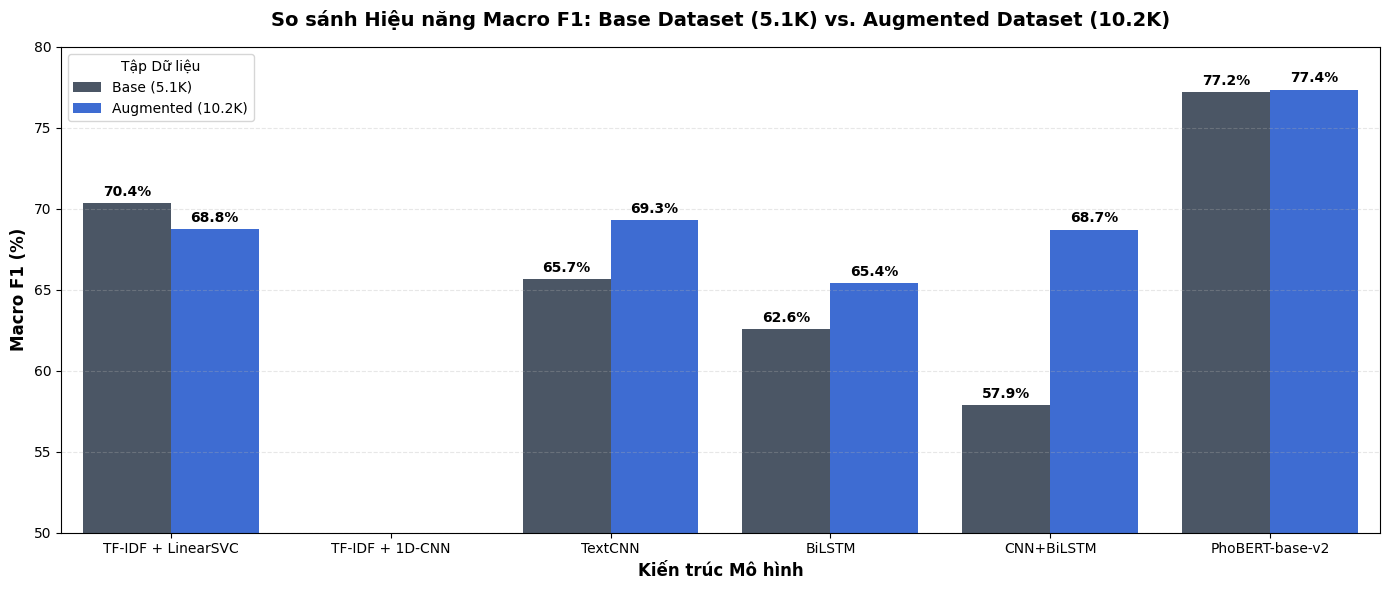
\includegraphics[width=0.88\textwidth]{figures/txt_model_comparison.png}
\caption{Biểu đồ cột đối chiếu Accuracy và Macro-F1 giữa 6 kiến trúc trên 2 cấu hình dữ liệu Base và Augmented (12 lượt chạy)}
\label{fig:txt_comp}
\end{figure}

\begin{table}[H]
\centering
\caption{Bảng phân tích mức độ hưởng lợi từ Tăng cường Dữ liệu (Augmentation Delta Gain)}
\label{tab:text_aug_gain}
\begin{tabular}{lrrrr}
\toprule
\textbf{Kiến trúc mô hình} & \textbf{Macro-F1 (Base)} & \textbf{Macro-F1 (Aug)} & \textbf{Chênh lệch ($\Delta$)} & \textbf{Tăng trưởng tương đối} \\
\midrule
\textbf{CNN + BiLSTM}      & 57{,}86\% & 68{,}71\% & \textbf{+10{,}85\%} & \textbf{+18{,}75\%} \\
TextCNN                    & 65{,}68\% & 69{,}31\% & +3{,}64\% & +5{,}54\% \\
BiLSTM                     & 62{,}58\% & 65{,}39\% & +2{,}81\% & +4{,}49\% \\
TF-IDF + 1D-CNN            & 16{,}68\% & 17{,}75\% & +1{,}07\% & +6{,}43\% \\
PhoBERT-base-v2            & 77{,}22\% & 77{,}36\% & +0{,}14\% & +0{,}18\% \\
TF-IDF + LinearSVC         & 70{,}36\% & 68{,}76\% & $-1{,}60\%$ & $-2{,}28\%$ \\
\bottomrule
\end{tabular}
\end{table}

\begin{figure}[H]
\centering
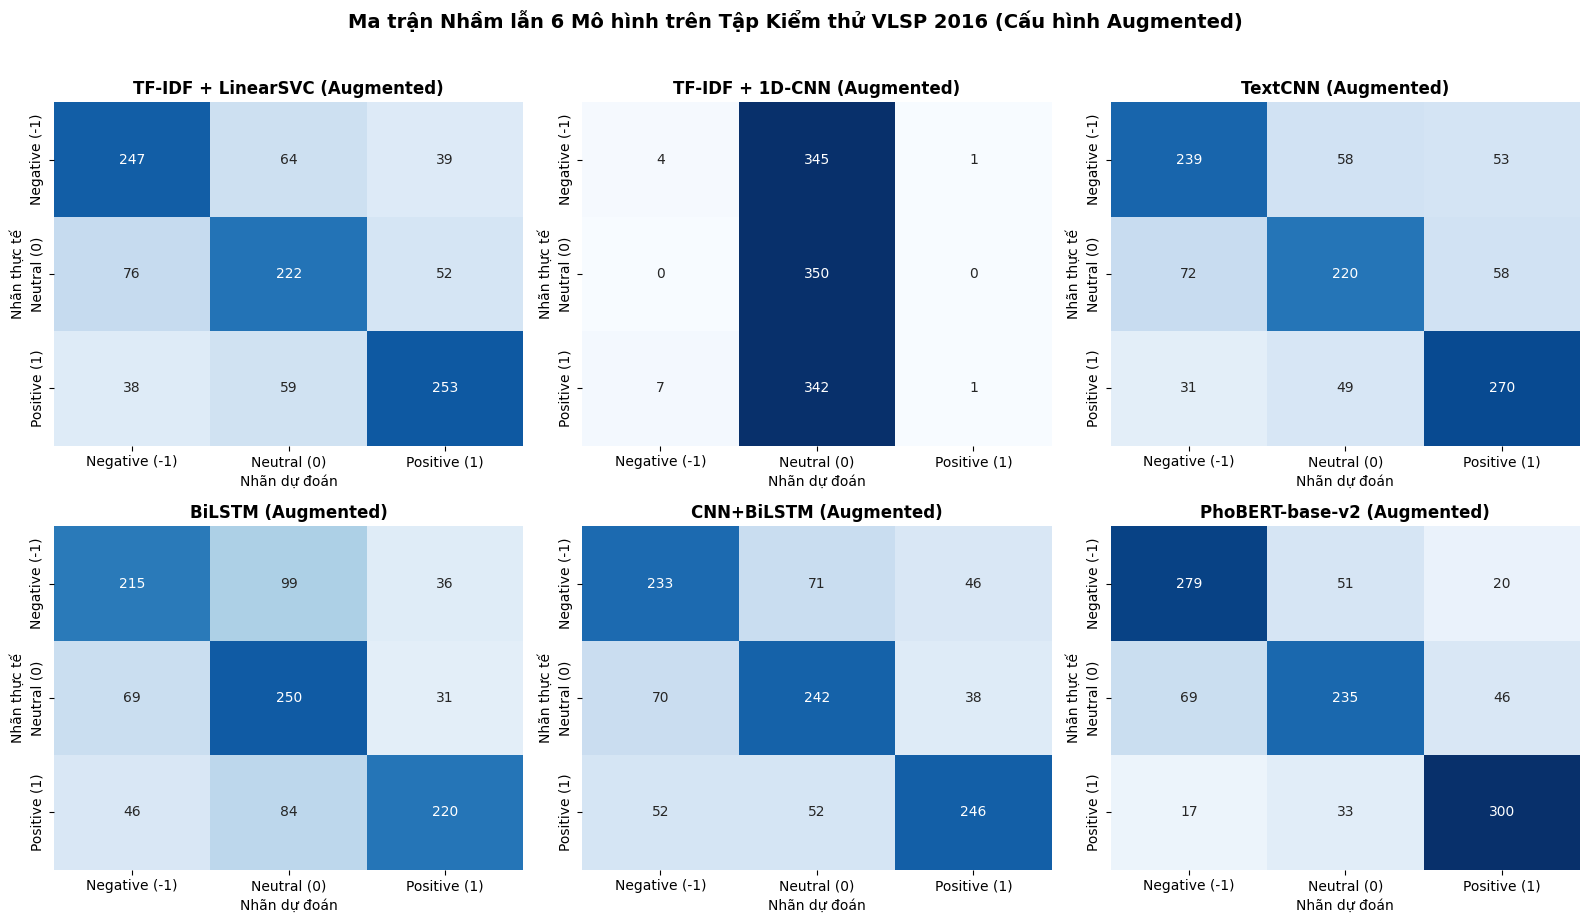
\includegraphics[width=0.92\textwidth]{figures/txt_confusion_matrices.png}
\caption{Lưới ma trận nhầm lẫn ($2 \times 3$) của 6 mô hình trên tập kiểm thử Test Set (1.050 mẫu)}
\label{fig:txt_cm}
\end{figure}

\subsubsection{Phân tích Chi tiết Lỗi theo Lớp của PhoBERT-base-v2}
Bảng \ref{tab:phobert_class} trình bày chi tiết hiệu năng theo từng lớp cảm xúc của mô hình dẫn đầu \textbf{PhoBERT-base-v2 (Augmented)}.

\begin{table}[H]
\centering
\caption{Hiệu năng phân loại theo từng lớp của PhoBERT-base-v2 (Augmented) trên tập Test}
\label{tab:phobert_class}
\begin{tabular}{lrrrrrr}
\toprule
\textbf{Lớp cảm xúc} & \textbf{Precision} & \textbf{Recall} & \textbf{F1-Score} & \textbf{Số mẫu test} & \textbf{Số mẫu sai} & \textbf{Tỷ lệ sai} \\
\midrule
Tiêu cực ($-1$) & 0{,}81 & 0{,}80 & 0{,}80 & 350 & 71 & 20{,}29\% \\
\textbf{Trung lập ($0$)} & \textbf{0{,}69} & \textbf{0{,}67} & \textbf{0{,}68} & \textbf{350} & \textbf{115} & \textbf{32{,}86\%} \\
Tích cực ($+1$) & 0{,}82 & 0{,}86 & 0{,}84 & 350 & 50 & 14{,}29\% \\
\bottomrule
\end{tabular}
\end{table}

\noindent \textbf{Khảo sát Định tính 5 Cơ chế Lỗi Ngôn ngữ Điển hình:}
Quan sát ma trận nhầm lẫn (Hình \ref{fig:txt_cm}) và phân tích mẫu lỗi (Bảng \ref{tab:phobert_class}) chỉ ra rằng \textbf{lớp Trung lập (0) là thách thức lớn nhất} với tỷ lệ dự đoán sai lên tới $32{,}86\%$ (115/350 mẫu). Nhóm phân loại các cơ chế lỗi bản chất thành 5 hiện tượng ngôn ngữ đặc thù:
\begin{enumerate}
    \item \textbf{Phân cực hai chiều (Dual Polarity):} Câu văn chứa cả khía cạnh khen lẫn chê (ví dụ: \textit{máy dùng mượt nhưng pin hơi yếu}). Nhãn thật là Trung lập (0), nhưng PhoBERT dự đoán thành Tiêu cực ($-1$) do bị chi phối bởi vế sau.
    \item \textbf{Lịch sự nghi thức (Social Courtesy):} Các câu chào hỏi, cảm ơn theo thói quen giao tiếp (ví dụ: \textit{cảm ơn shop đã giao hàng}). Nhãn thật là Trung lập (0), nhưng mô hình bị các từ mang sắc thái tích cực đánh lừa thành Tích cực ($+1$).
    \item \textbf{Trần thuật thông số kỹ thuật (Factual Reporting):} Các câu thuần túy liệt kê sự việc (ví dụ: \textit{đã nhận máy màu xanh 128gb}). Nhãn thật là Trung lập (0), nhưng mô hình dễ bị gán nhầm sang Tích cực ($+1$).
    \item \textbf{Than phiền ngầm (Implicit Complaint):} Câu phàn nàn không dùng từ ngữ tiêu cực trực diện (ví dụ: \textit{đóng gói thế này thì cũng chịu}). Nhãn thật là Tiêu cực ($-1$), nhưng mô hình nhận diện là Trung lập (0).
    \item \textbf{Châm biếm và Mỉa mai (Sarcasm / Irony):} Sử dụng từ tích cực để diễn đạt ý tiêu cực (ví dụ: \textit{mượt ghê văng luôn ứng dụng}). Nhãn thật là Tiêu cực ($-1$), nhưng mô hình dự đoán nhầm thành Tích cực ($+1$).
\end{enumerate}

\noindent \textbf{Thảo luận Tổng kết Thực nghiệm Text:}
\begin{itemize}
    \item \textbf{Ưu thế của Transformer tiền huấn luyện:} PhoBERT-base-v2 đạt hiệu năng quán quân trên cả hai tập dữ liệu (Test Accuracy $77{,}52\%$, Macro-F1 $0{,}7736$). Cơ chế Self-Attention đa tầng được tiền huấn luyện trên kho ngữ liệu tiếng Việt lớn nắm bắt rất chuẩn xác mối liên kết ngữ nghĩa giữa các từ ghép.
    \item \textbf{Sự phân hóa khi Tăng cường Dữ liệu (Augmentation):} Tăng cường dữ liệu bằng dịch vòng (Back-translation) đem lại bước nhảy vọt ngoạn mục cho mô hình lai ghép CNN+BiLSTM ($+10{,}85\%$ Macro-F1) và TextCNN ($+3{,}64\%$). Ngược lại, TF-IDF + LinearSVC bị giảm nhẹ $-1{,}60\%$ do câu dịch vòng làm loãng tần suất các n-gram từ khóa chính xác.
    \item \textbf{Thất bại của 1D-CNN trên TF-IDF:} TF-IDF + 1D-CNN chỉ đạt Accuracy $\approx 33{,}81\%$ và Macro-F1 $0{,}1775$ (tương đương đoán ngẫu nhiên), chứng minh phép tích chập không gian không thể học được đặc trưng trên một vector tần suất từ ngữ thưa thớt vốn không có trật tự thời gian.
\end{itemize}

% ==============================================================================
% SECTION 4: GENERAL CONCLUSION
% ==============================================================================
\newpage
\section{Kết luận Toàn diện Đồ án và Đóng góp Nhóm}

\subsection{Tổng kết Quy trình Kỹ thuật}
Qua đồ án môn học \textbf{CO5177}, nhóm \textbf{SlightSeek} đã hoàn thiện quy trình khoa học dữ liệu bài bản trên cả ba dạng thức dữ liệu trọng tâm:
\begin{enumerate}
    \item \textbf{Dữ liệu Bảng (Adult Census Income):} Thực hiện EDA hai tầng, xử lý triệt để bài toán mất cân bằng lớp và dữ liệu thiếu, xây dựng pipeline đặc trưng tối ưu và chứng minh tính ưu việt của mô hình XGBoost ($ROC\text{-}AUC = 0{,}9267$).
    \item \textbf{Dữ liệu Ảnh (Intel Image Classification):} Khử trùng lặp pixel RGB, thiết lập quy trình Transfer Learning hai giai đoạn với MobileNetV3-Small và ViT-B/16, chỉ ra cơ chế Attention của Vision Transformer mang lại chất lượng vượt trội ($94{,}50\%$ Test Accuracy).
    \item \textbf{Dữ liệu Văn bản (VLSP 2016 Sentiment):} Xử lý ngôn ngữ tự nhiên tiếng Việt qua chuẩn hóa Teencode, từ điển Emoticons, tách từ BPE/PyVi, đối chứng toàn diện 12 thực nghiệm trên 6 kiến trúc (TF-IDF, Word2Vec CBOW, và PhoBERT-base-v2) trên cả hai cấu hình Base và Augmented, đạt đỉnh cao với PhoBERT-base-v2 ($77{,}52\%$ Test Accuracy và $0{,}7736$ Macro-F1).
\end{enumerate}

Toàn bộ quy trình được bảo đảm nghiêm ngặt về tính tái lập (\textit{Reproducibility}), cố định random seed và cam kết chống rò rỉ thông tin (\textit{No Data Leakage}) giữa các phân tập dữ liệu.

\subsection{Bảng Phân công và Đóng góp của Thành viên Nhóm}
\begin{table}[H]
\centering
\caption{Bảng phân công nhiệm vụ và tỷ lệ hoàn thành công việc của nhóm SlightSeek}
\begin{tabularx}{\textwidth}{p{4cm} c X c}
\toprule
\textbf{Thành viên} & \textbf{MSSV} & \textbf{Nhiệm vụ chính phụ trách} & \textbf{Đóng góp} \\
\midrule
\textbf{Phạm Duy Anh} & 2310139 & 
- Xây dựng pipeline Image (MobileNetV3 \& ViT-B/16), EDA và chống rò rỉ. \newline
- Huấn luyện và fine-tune PhoBERT-base-v2 (Base \& Augmented) cho Text Sentiment. \newline
- Thiết kế hệ thống web GitHub Pages và đồng bộ hóa báo cáo LaTeX. & 100\% \\
\midrule
\textbf{Nguyễn Phan Tuấn Duy} & 2310491 & 
- Xây dựng pipeline Tabular (EDA 2 lần, Feature Selection, 5 mô hình ML). \newline
- Xây dựng các mô hình TF-IDF \& Word2Vec (LinearSVC, 1D-CNN, TextCNN, BiLSTM, CNN+BiLSTM) cho Text. \newline
- Thu thập tài liệu tham khảo và viết nội dung phân tích Tabular. & 100\% \\
\bottomrule
\end{tabularx}
\end{table}

\newpage
\bibliographystyle{IEEEtran}
\bibliography{refs}

\end{document}
